\chapter{Alkalmazás működése}

A következőkben az alkalmazás funkcióit fogom bemutatni, a leírásokat képernyőképekkel kiegészítve. A képek néhol eltérnek egymástól, melynek oka hogy az applikáció funkcionalitásából fakadóan nem volt lehetséges mindet az emulátoron elkészíteni, hanem a jegyzetek készítéséhez fizikai készülékre is szükség volt.

\section{Bejelentkezés}
A telepítést követően a bejelentkezési képernyő az első, amivel a felhasználó találkozik. Ez már korábban megjelent a dolgozatban, a \refstruc{fig:MaterialBeforeAfter} bemutatásában. Itt a beviteli mezők segédszövegei egyértelműsítik, hogy milyen adatok elvártak a bejelentkezéshez illetve regisztrációhoz. Ezek gombnyomás hatására validálásra kerülnek, és amennyiben az e-mail formátuma nem érvényes vagy a jelszó hossza nem éri el a 6 karaktert, akkor a folyamat meghiúsul, és a felhasználó értesül róla, hogy mely mező(k) tartalmát kell javítania.

\section{Kategorizált lista}
Sikeres bejelentkezést követően az alkalmazás a fő képernyőjére navigál, ahol az eddig elmentett jegyzeteket láthatjuk kategóriákba rendezve. A kategóriák alapértelmezetten össze vannak csukva, csak a legfelső szinten található elemeket látjuk. A lista sorainak jobb szélén elhelyezkedő nyilakra kattintva tudjuk kibontani az adott kategóriát, ezzel megtekinteni a tartalmát (\refstruc{fig:NoteListScreen}).

\begin{figure}[!ht]
	\centering
	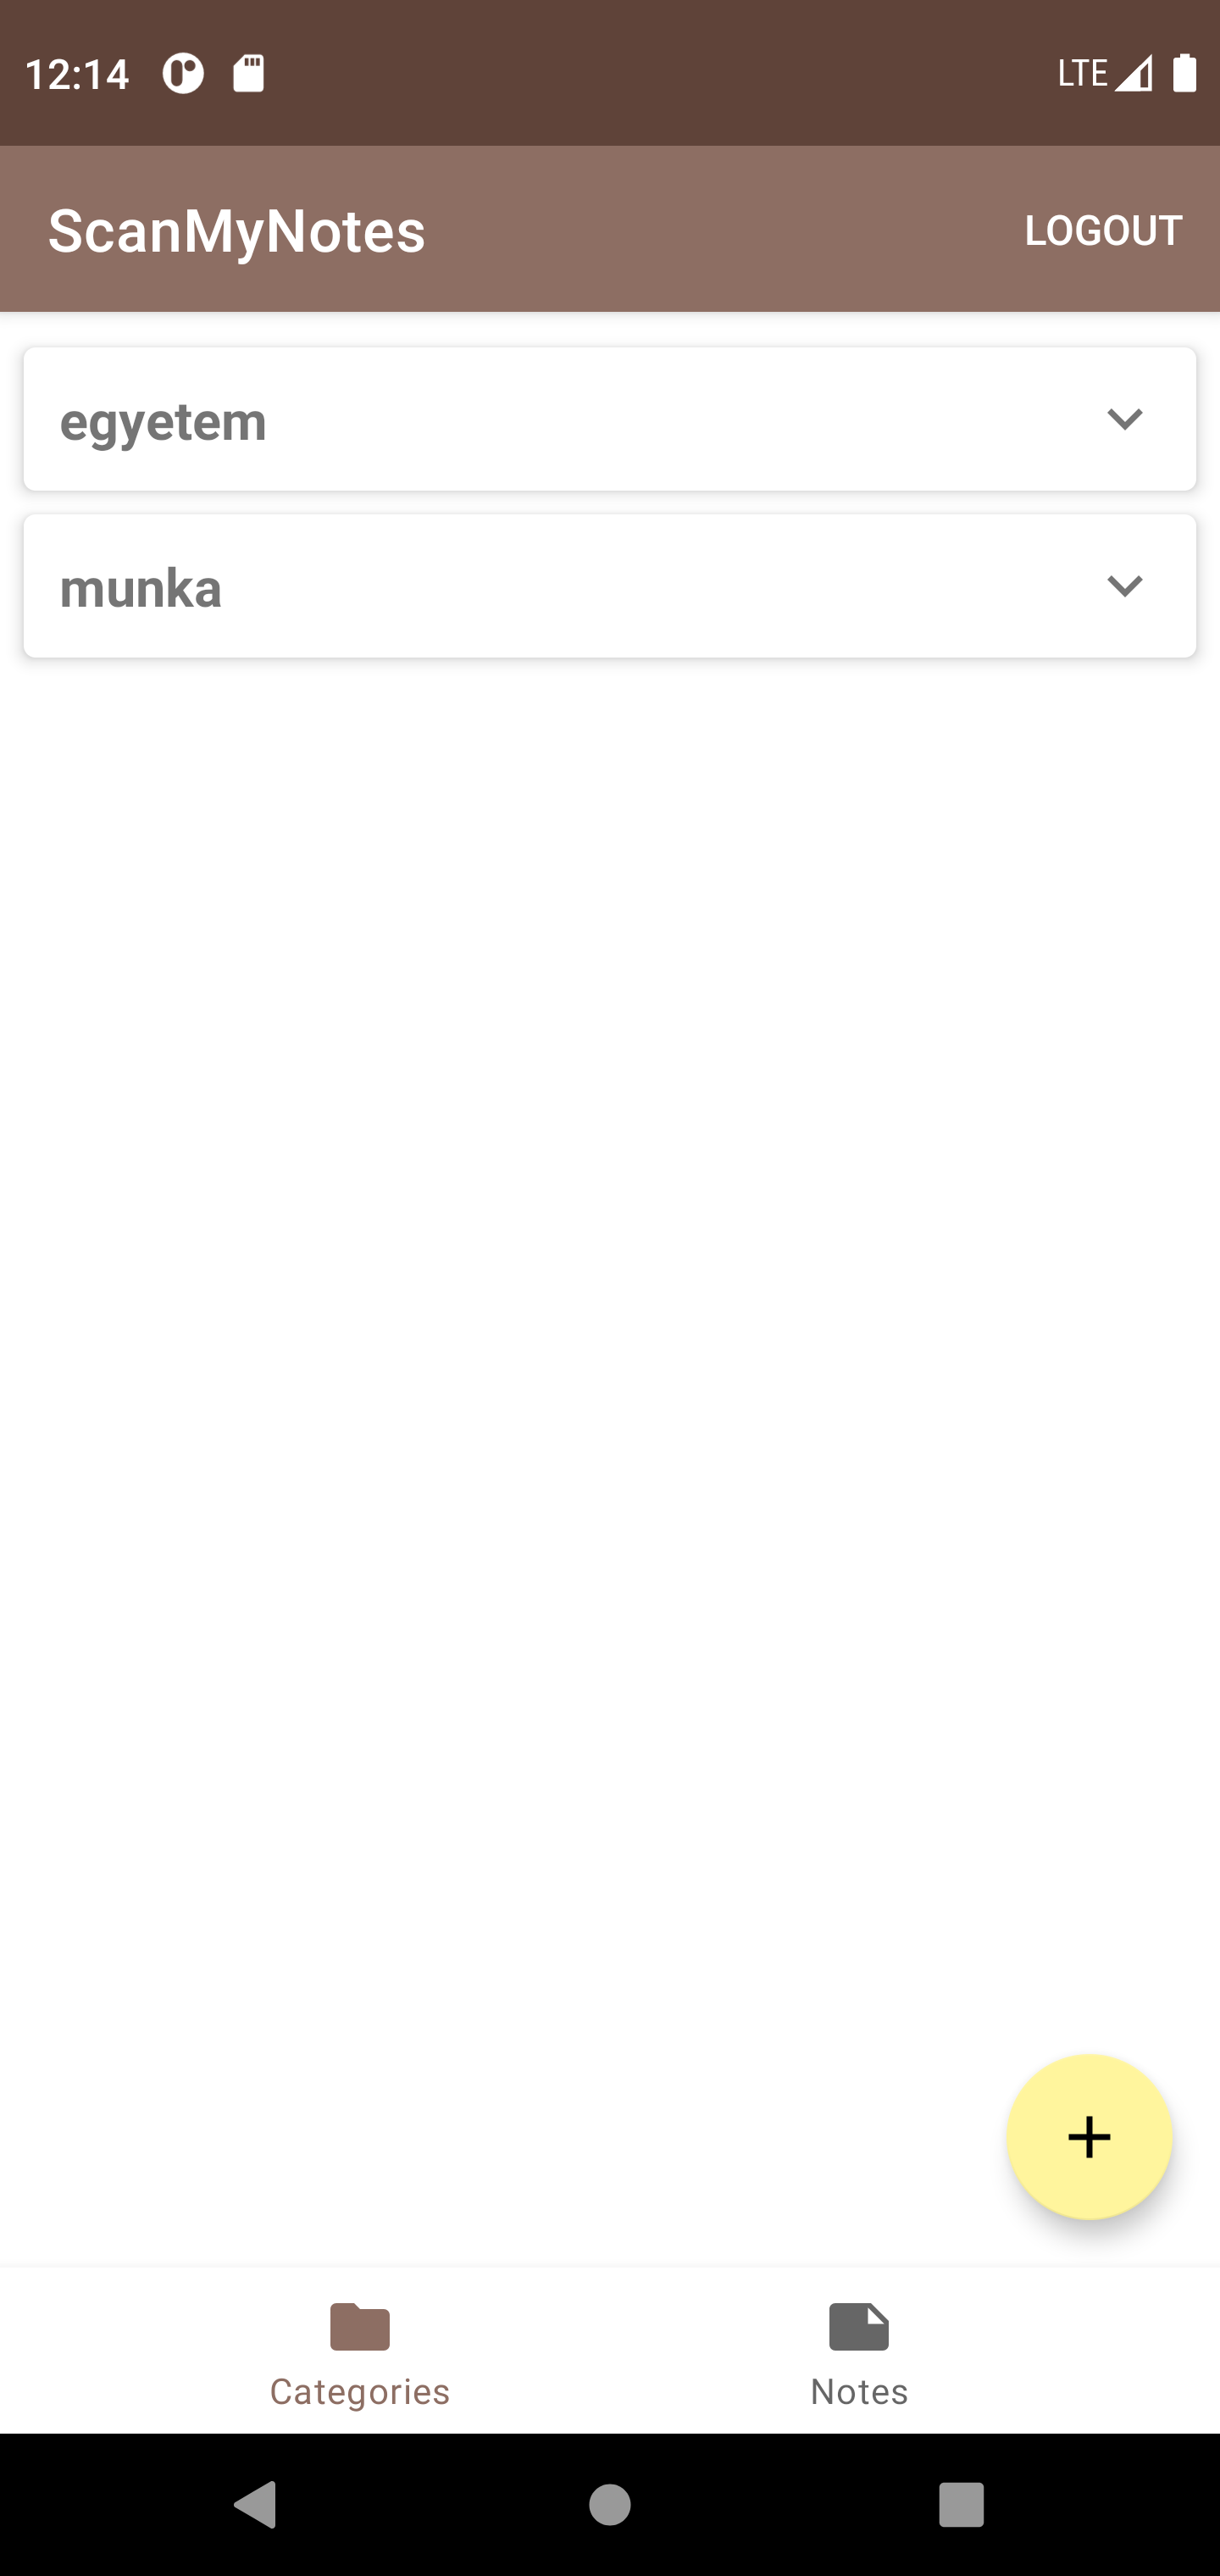
\includegraphics[width=55mm, keepaspectratio]{figures/notelist_closed.png}
	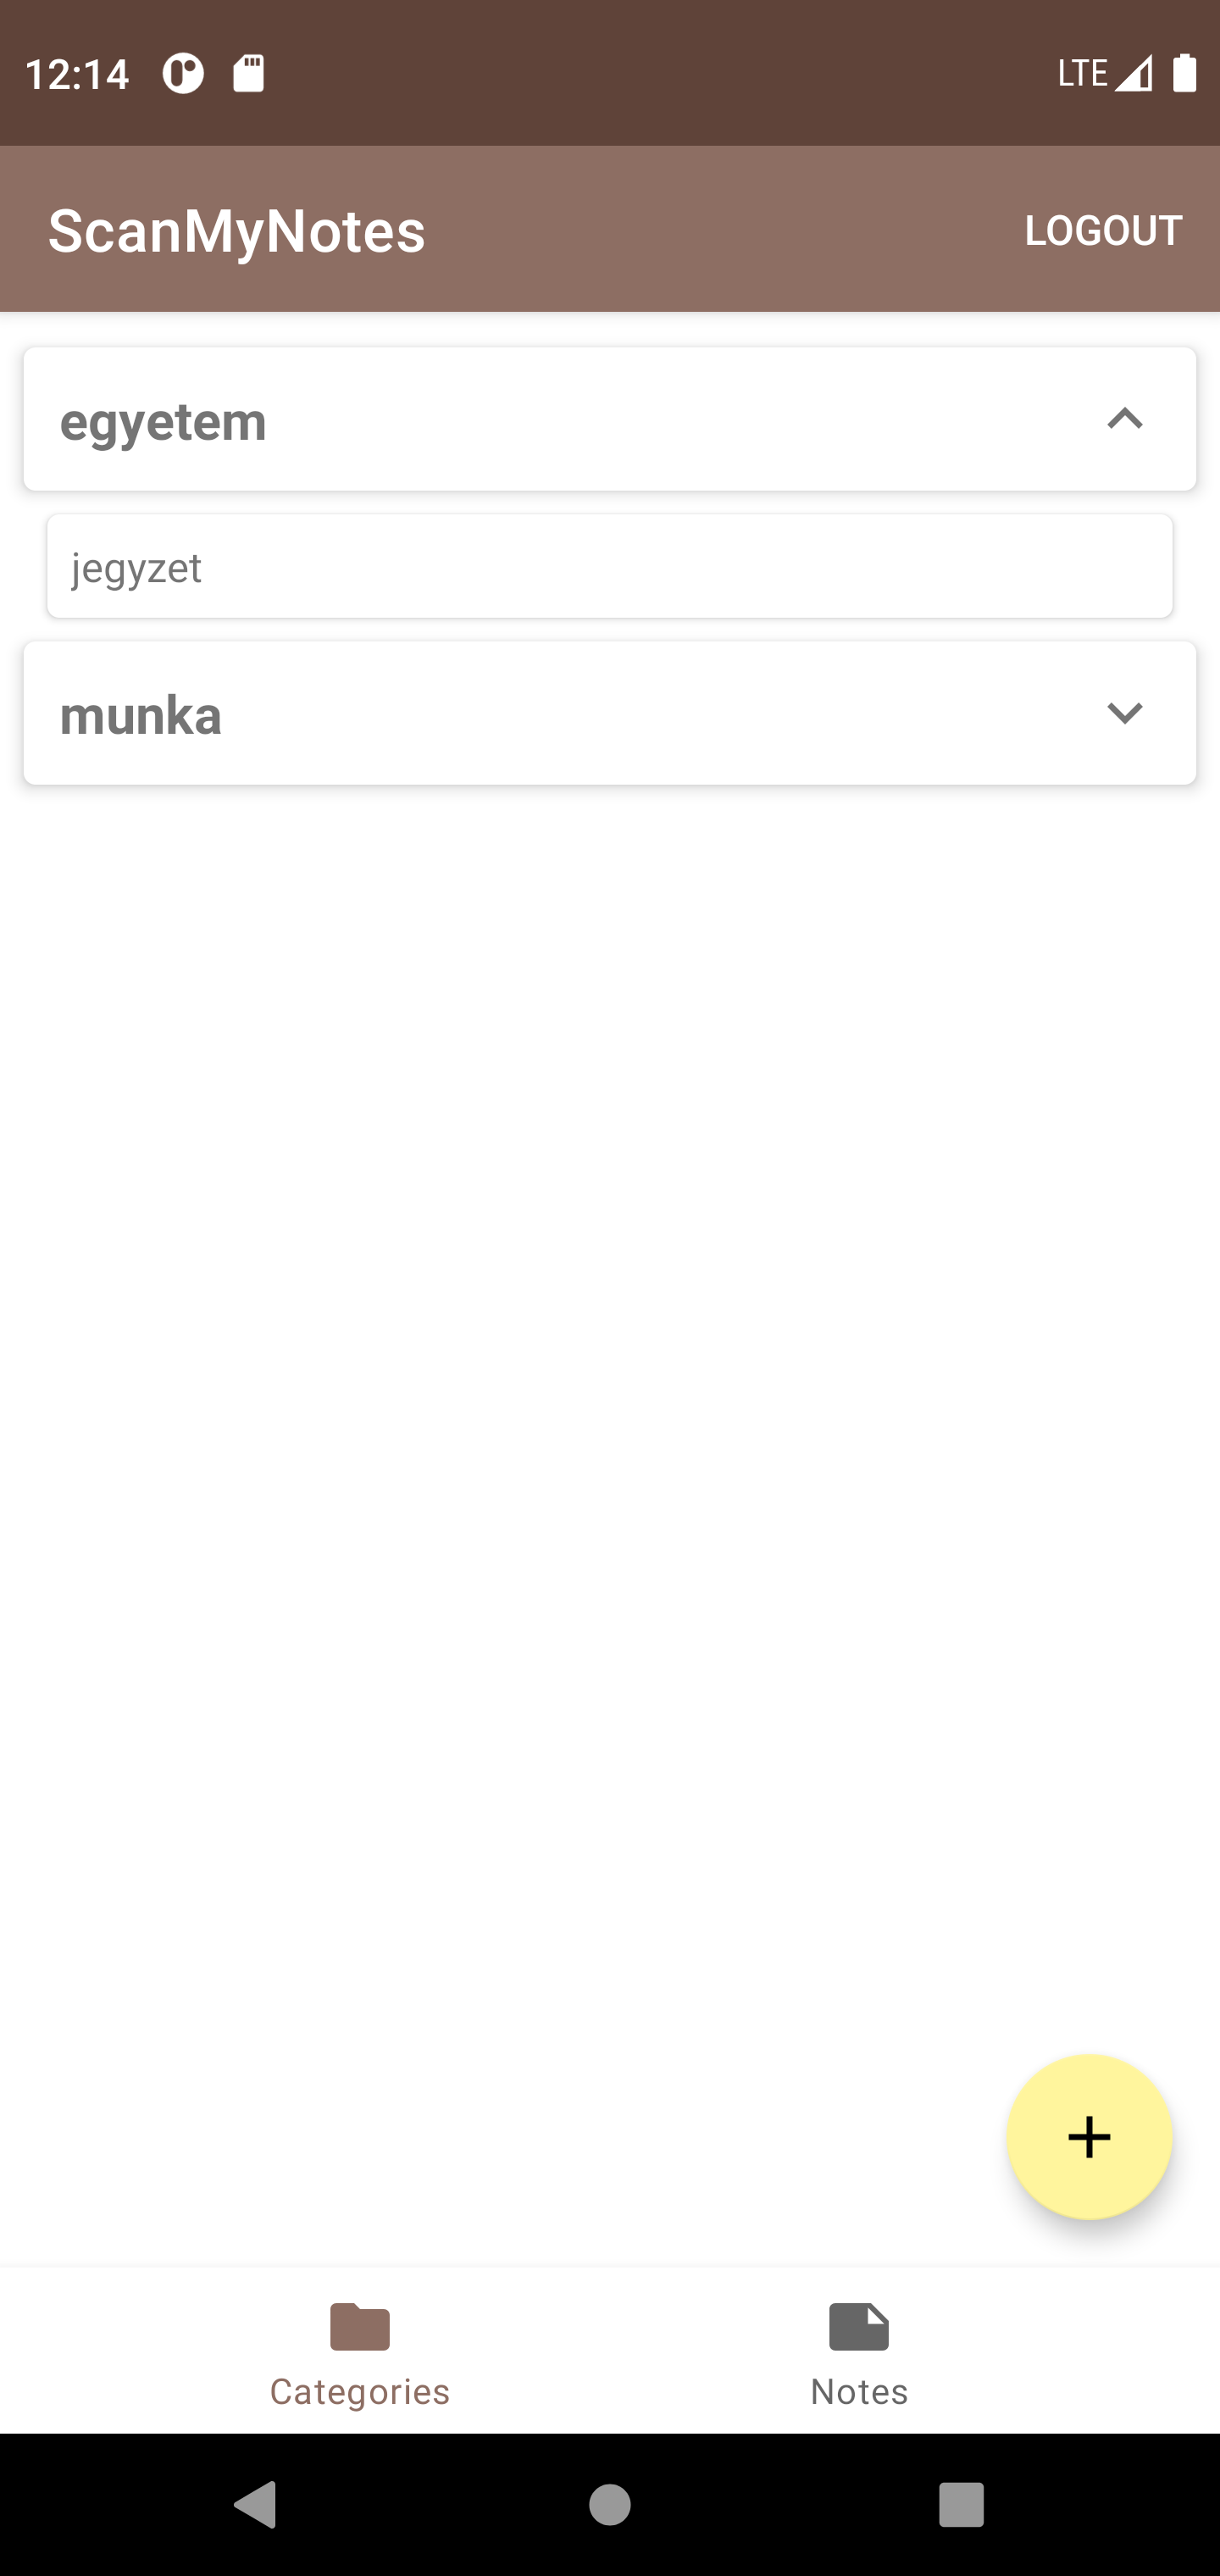
\includegraphics[width=55mm, keepaspectratio]{figures/notelist_open.png}
	\caption{Az alkalmazás kezdőlapja alapértelmezett állapotban, illetve egy kategória kibontva.}
	\label{fig:NoteListScreen}
\end{figure}

Innen számos lehetőségünk adódik navigációra az applikáción belül, kezdve a jobb felső sarokban található, meglehetősen magától értetődő kijelentkezés gombbal. Ezt megnyomva a fent leírt bejelentkezési képernyőre navigálunk, ahol adataink megadásával újra bejelentkezhetünk.

\section{Jegyzetlista}
A főképernyőn alul egy navigációs sávot találunk, mellyel a két különböző listamegjelenítés között tudunk váltani. Míg a \emph{Categories} opció alatt egy hierarchikusan egymás alá rendezett listát láthatunk, a \emph{Notes} opció csak a jegyzeteket tárja elénk, kategóriától függetlenül. Itt több lehetőség tárul elénk: a képernyő tetején található egy keresősáv és egy rendezés gomb. Keresni a jegyzetek címe alapján tudunk, itt gépelés közben azonnal szűkül az eredményhalmaz. A rendezés szintén a cím alapján működik, jelenleg növekvő és csökkenő betűrendet támogat az alkalmazás (\refstruc{fig:NoteListScreen2}).

\begin{figure}[!ht]
	\centering
	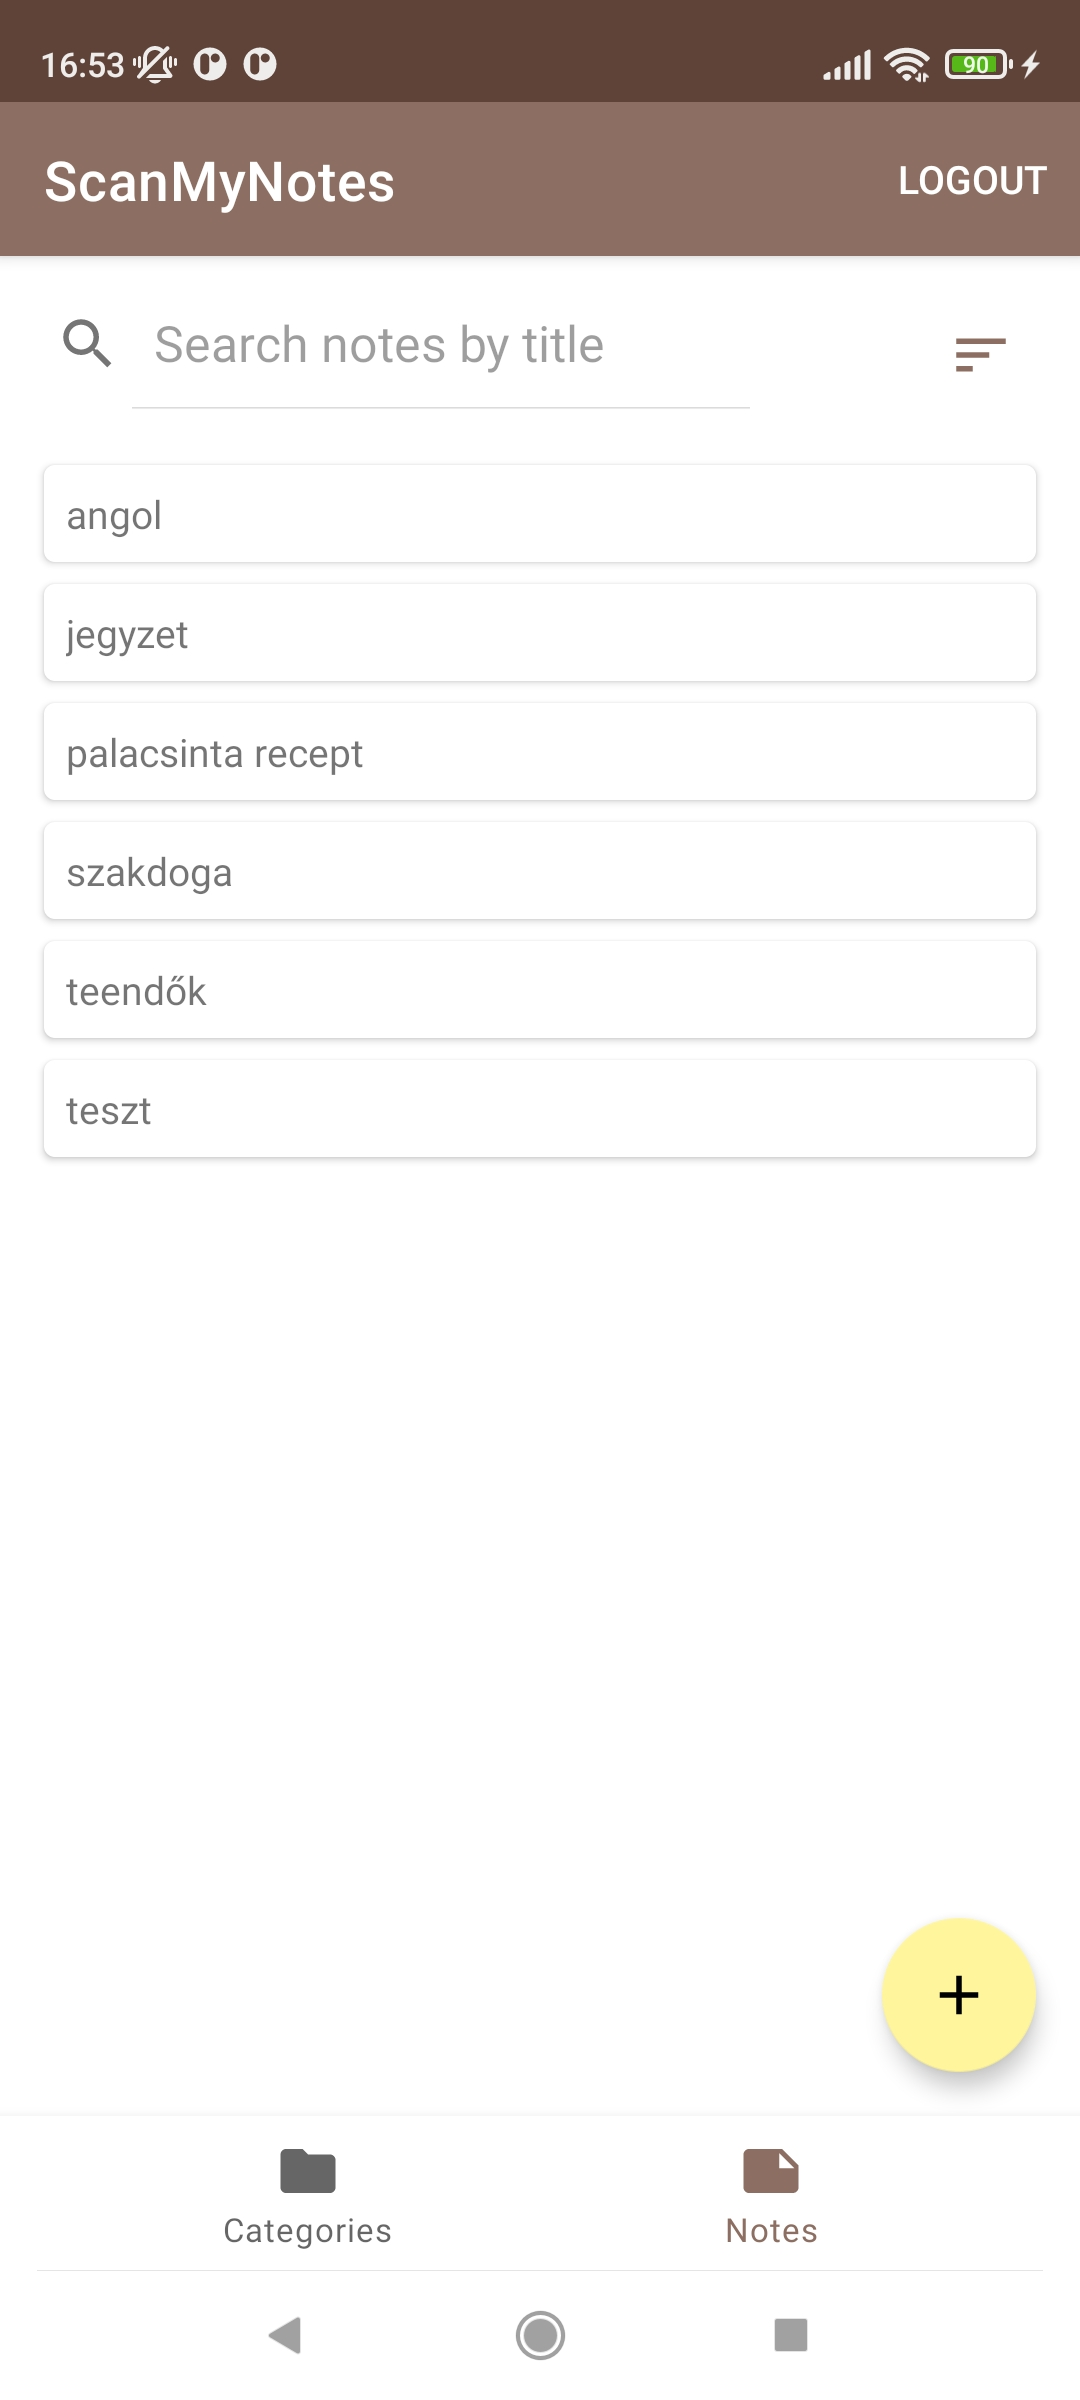
\includegraphics[width=49mm, keepaspectratio]{figures/notelist_full.jpg}
	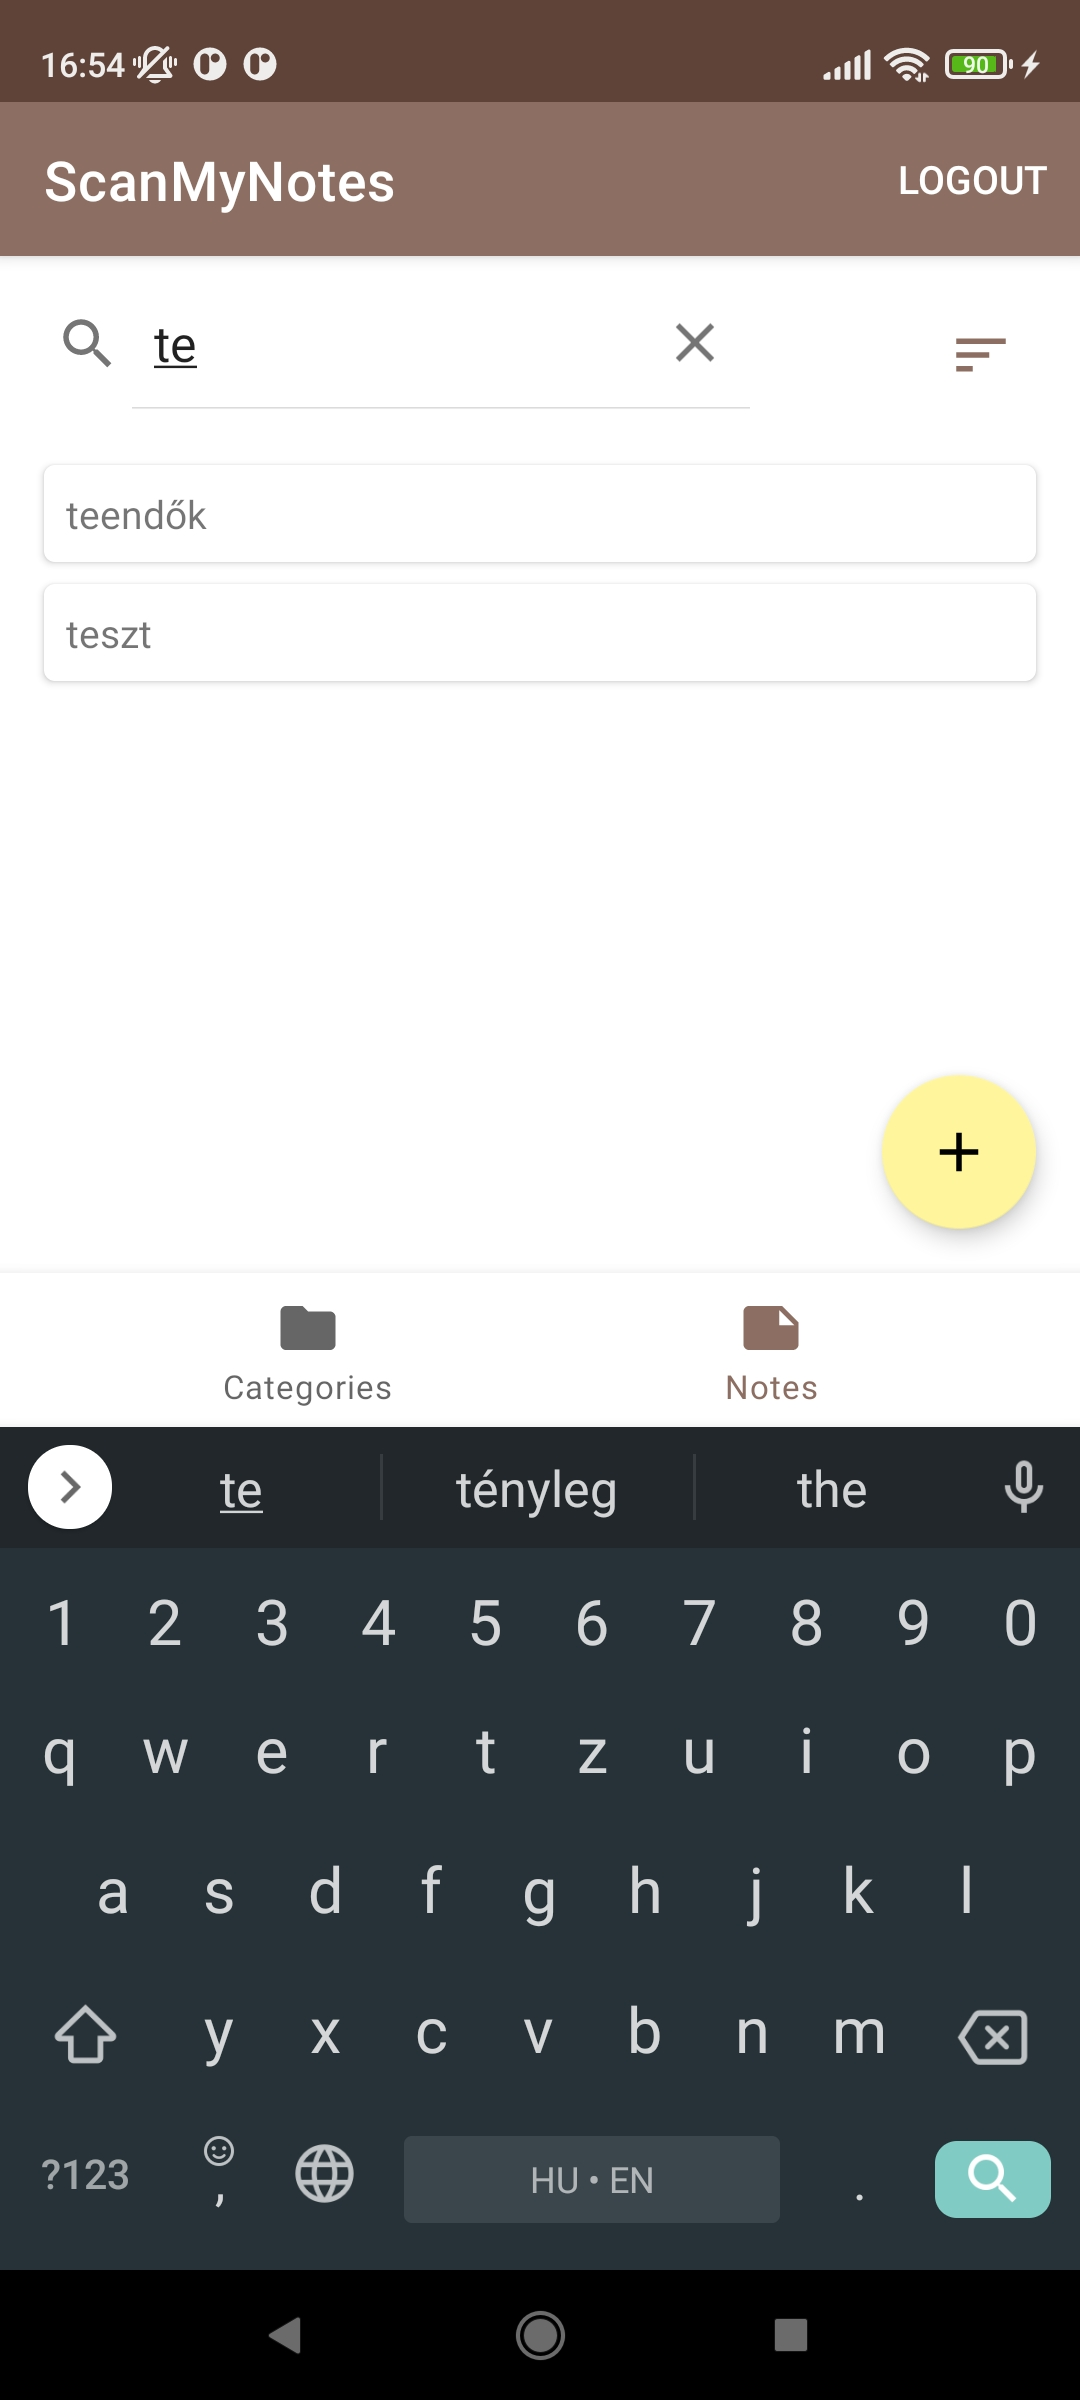
\includegraphics[width=49mm, keepaspectratio]{figures/notelist_search.jpg}
	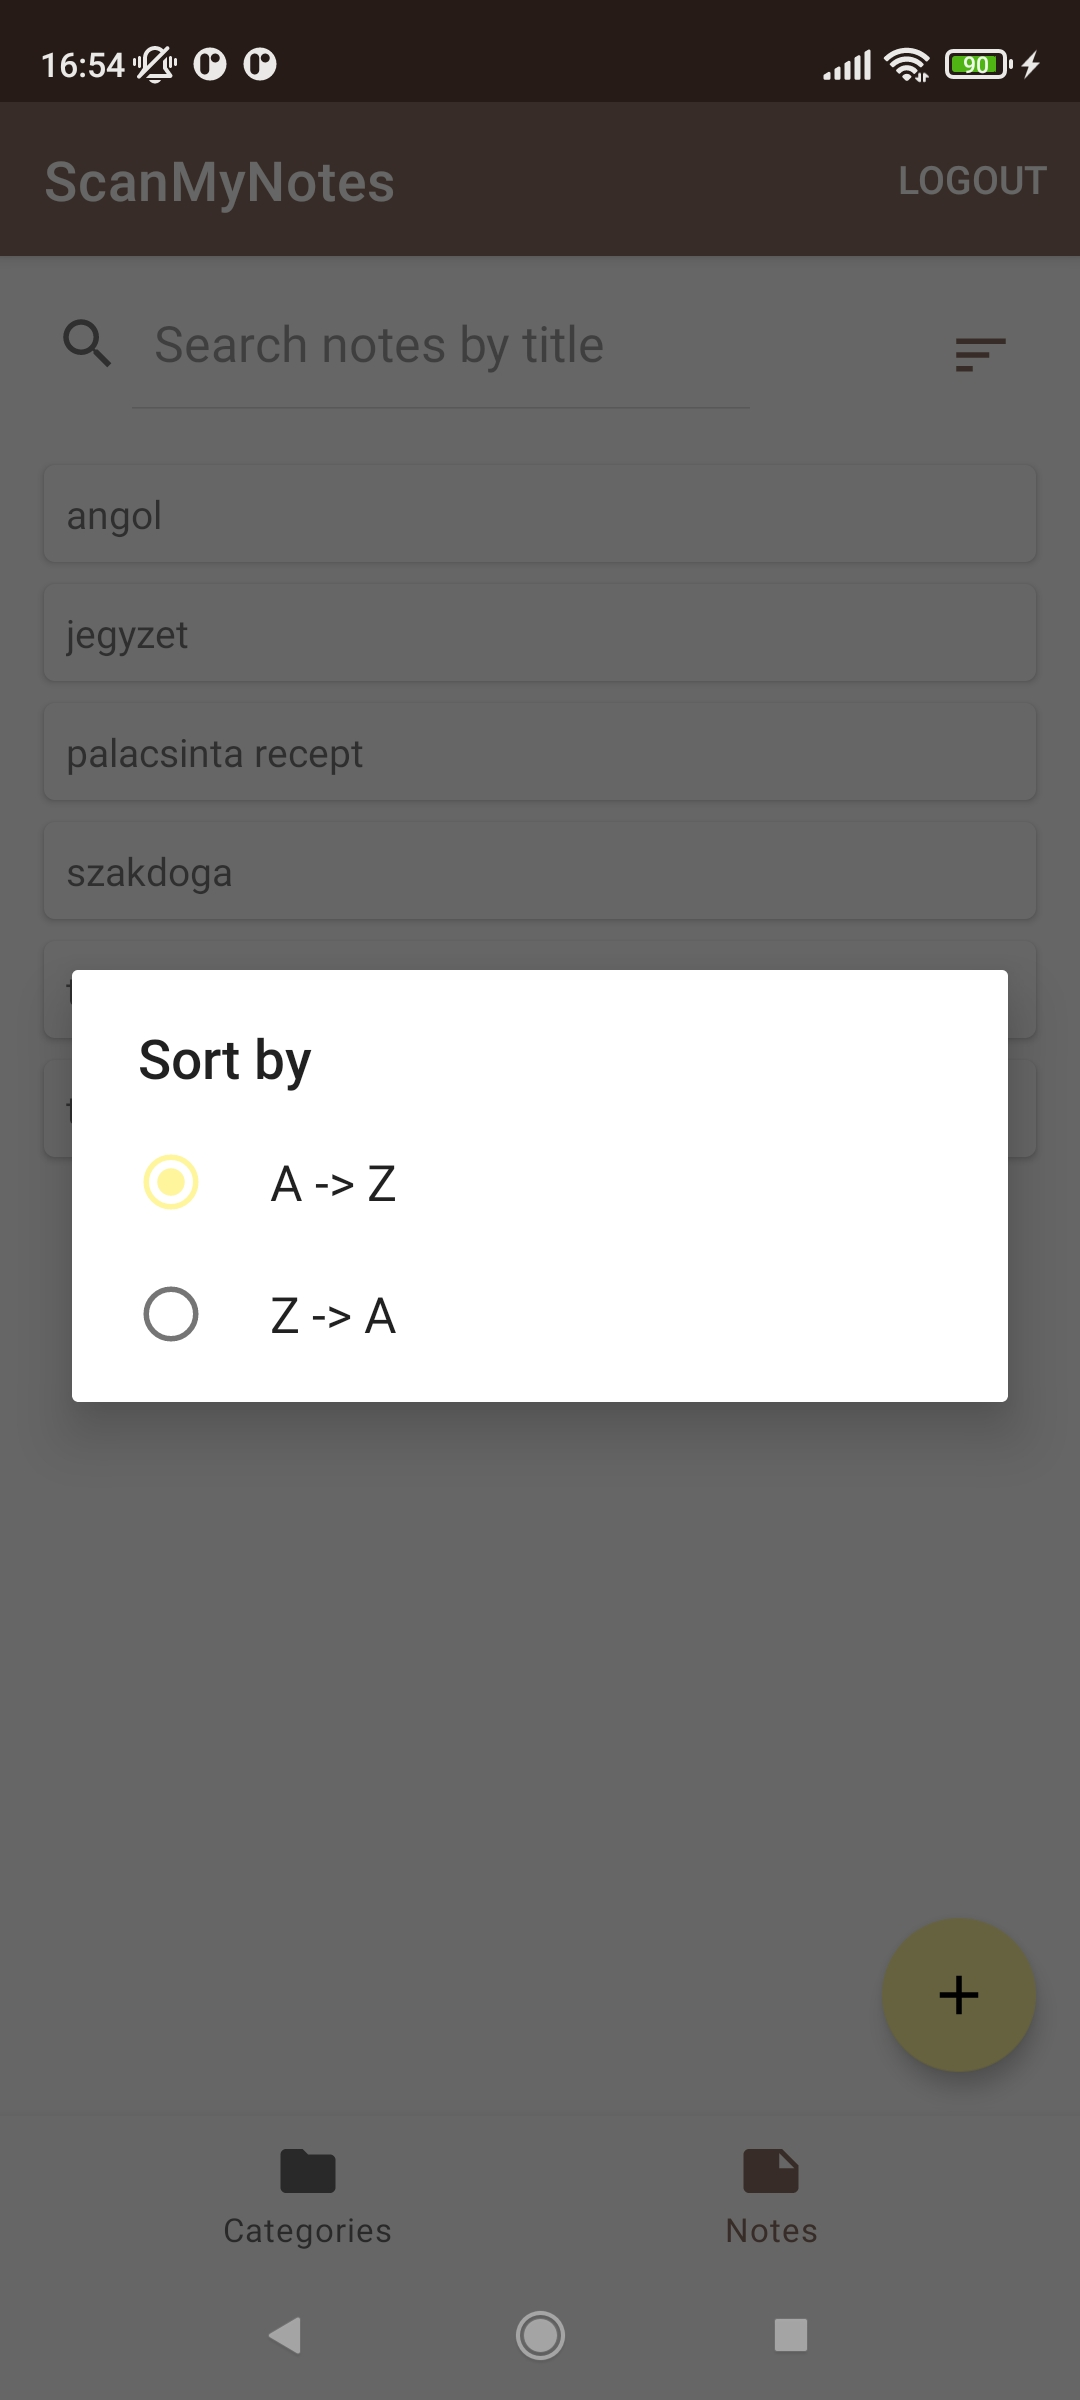
\includegraphics[width=49mm, keepaspectratio]{figures/notelist_sort.jpg}
	\caption{A jegyzetek listája, és a rajta elvégezhető műveletek.}
	\label{fig:NoteListScreen2}
\end{figure}

\section{Jegyzet létrehozása}
Az alkalmazás fő funkcionalitása a jegyzetek tárolása, így elég fontos, hogy legyen lehetőség újak létrehozására. Ez a képernyő jobb alsó sarkában található plusz gombra kattintva tehető meg. Az ott megjelenő két újabb gomb közül az alsó megnyomására felugrik egy kameraablak, ahol egy fénykép készítése után megtörténik a digitalizáció, és a szerkesztési oldalra ugrunk. Itt egy cím megadásával fejezhetjük be a létrehozási folyamatot, de opcionálisan hozzárendelhetjük egy kategóriához is (\refstruc{fig:NewNoteScreen}). Amíg a cím vagy a tartalom üres, addig az alkalmazás nem fogja engedni elmenteni a jegyzetet, figyelmeztetést rak az üresen hagyott mezőre.
\begin{figure}[!ht]
	\centering
	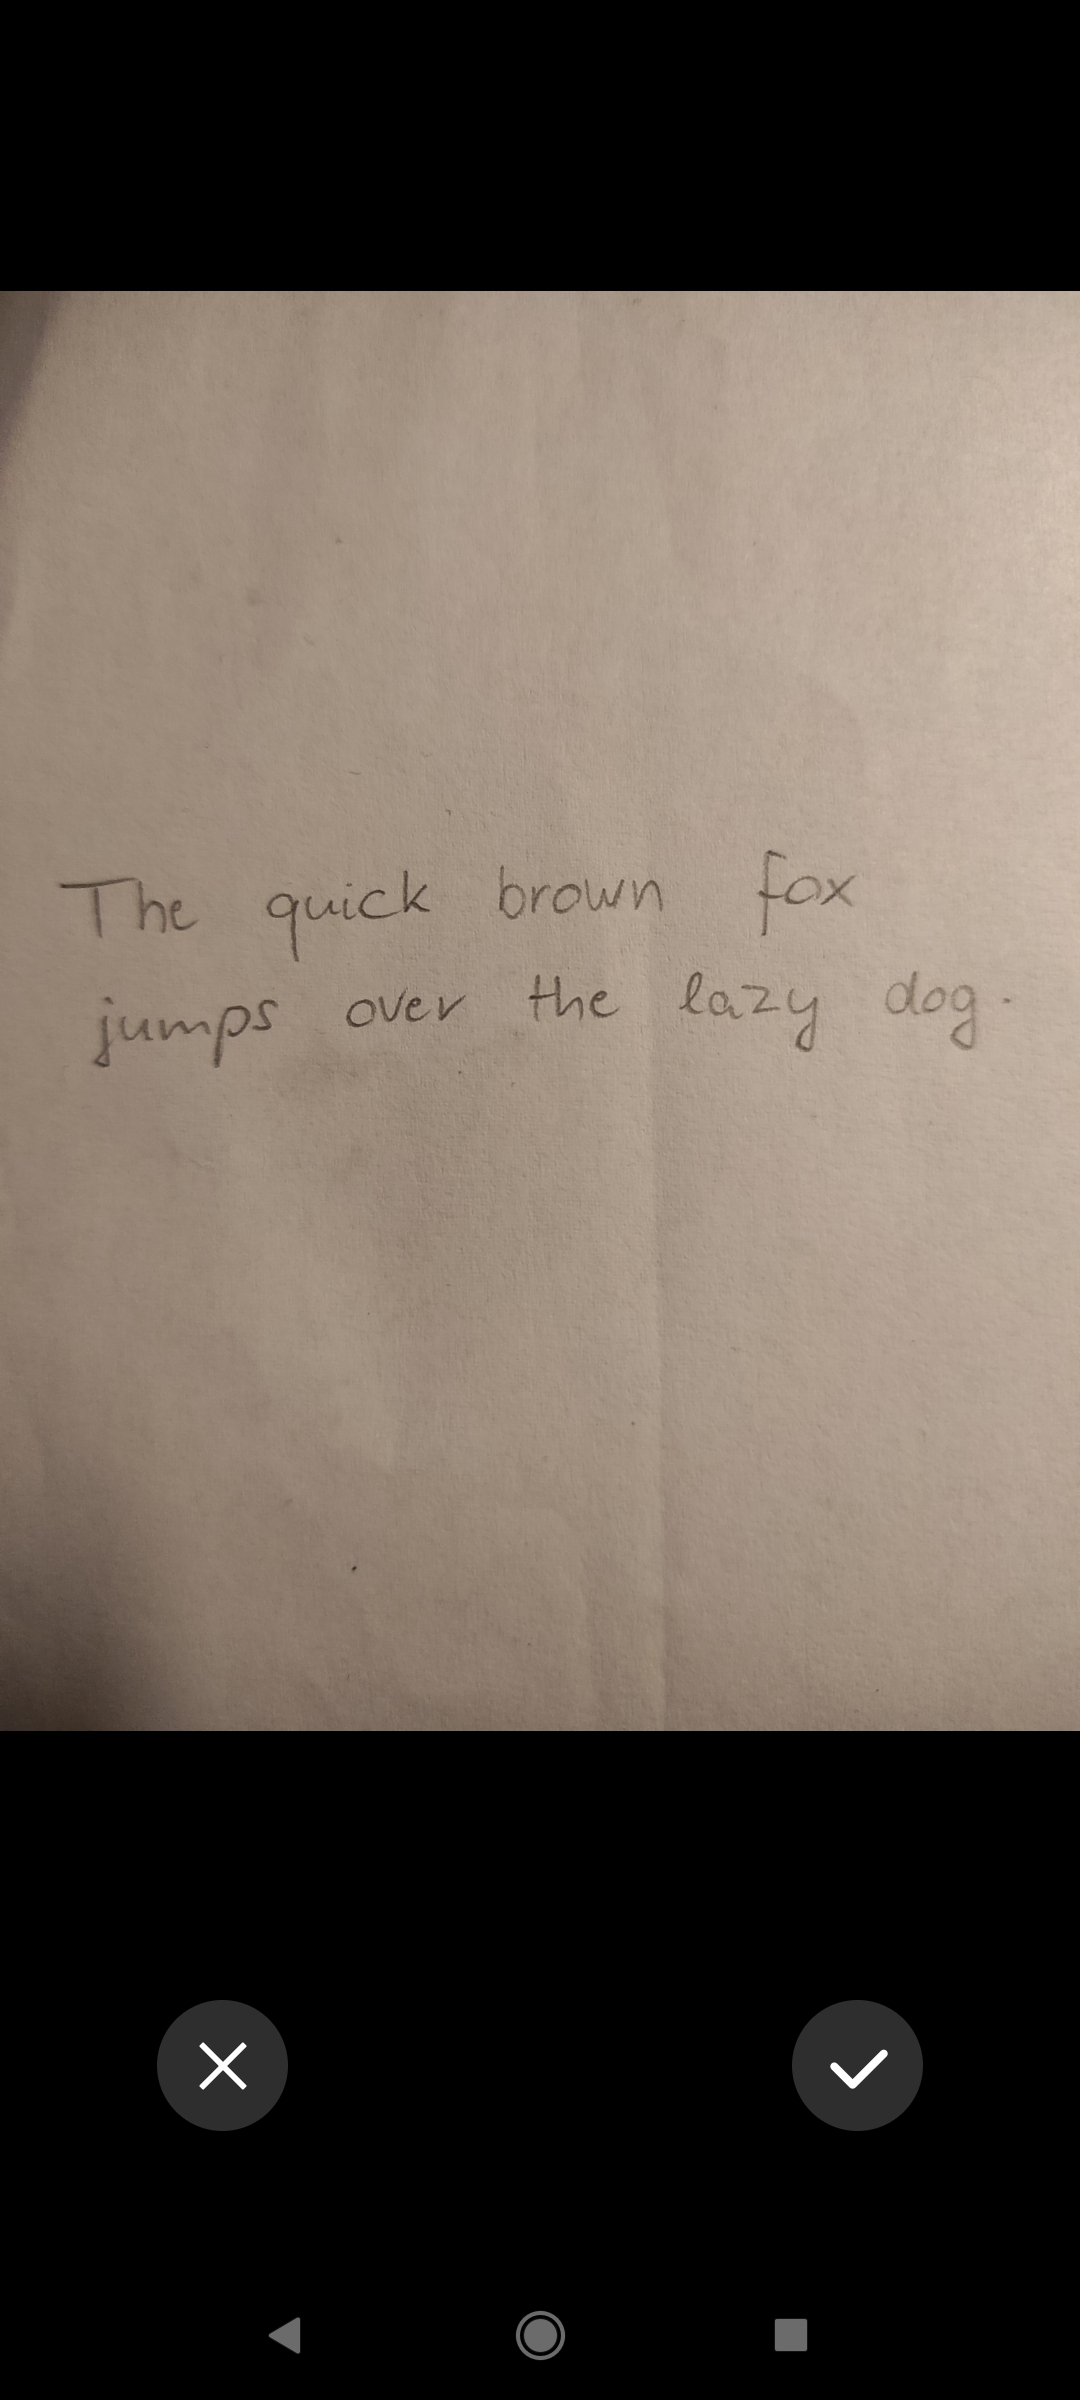
\includegraphics[width=55mm, keepaspectratio]{figures/newnote_photo.jpg}
	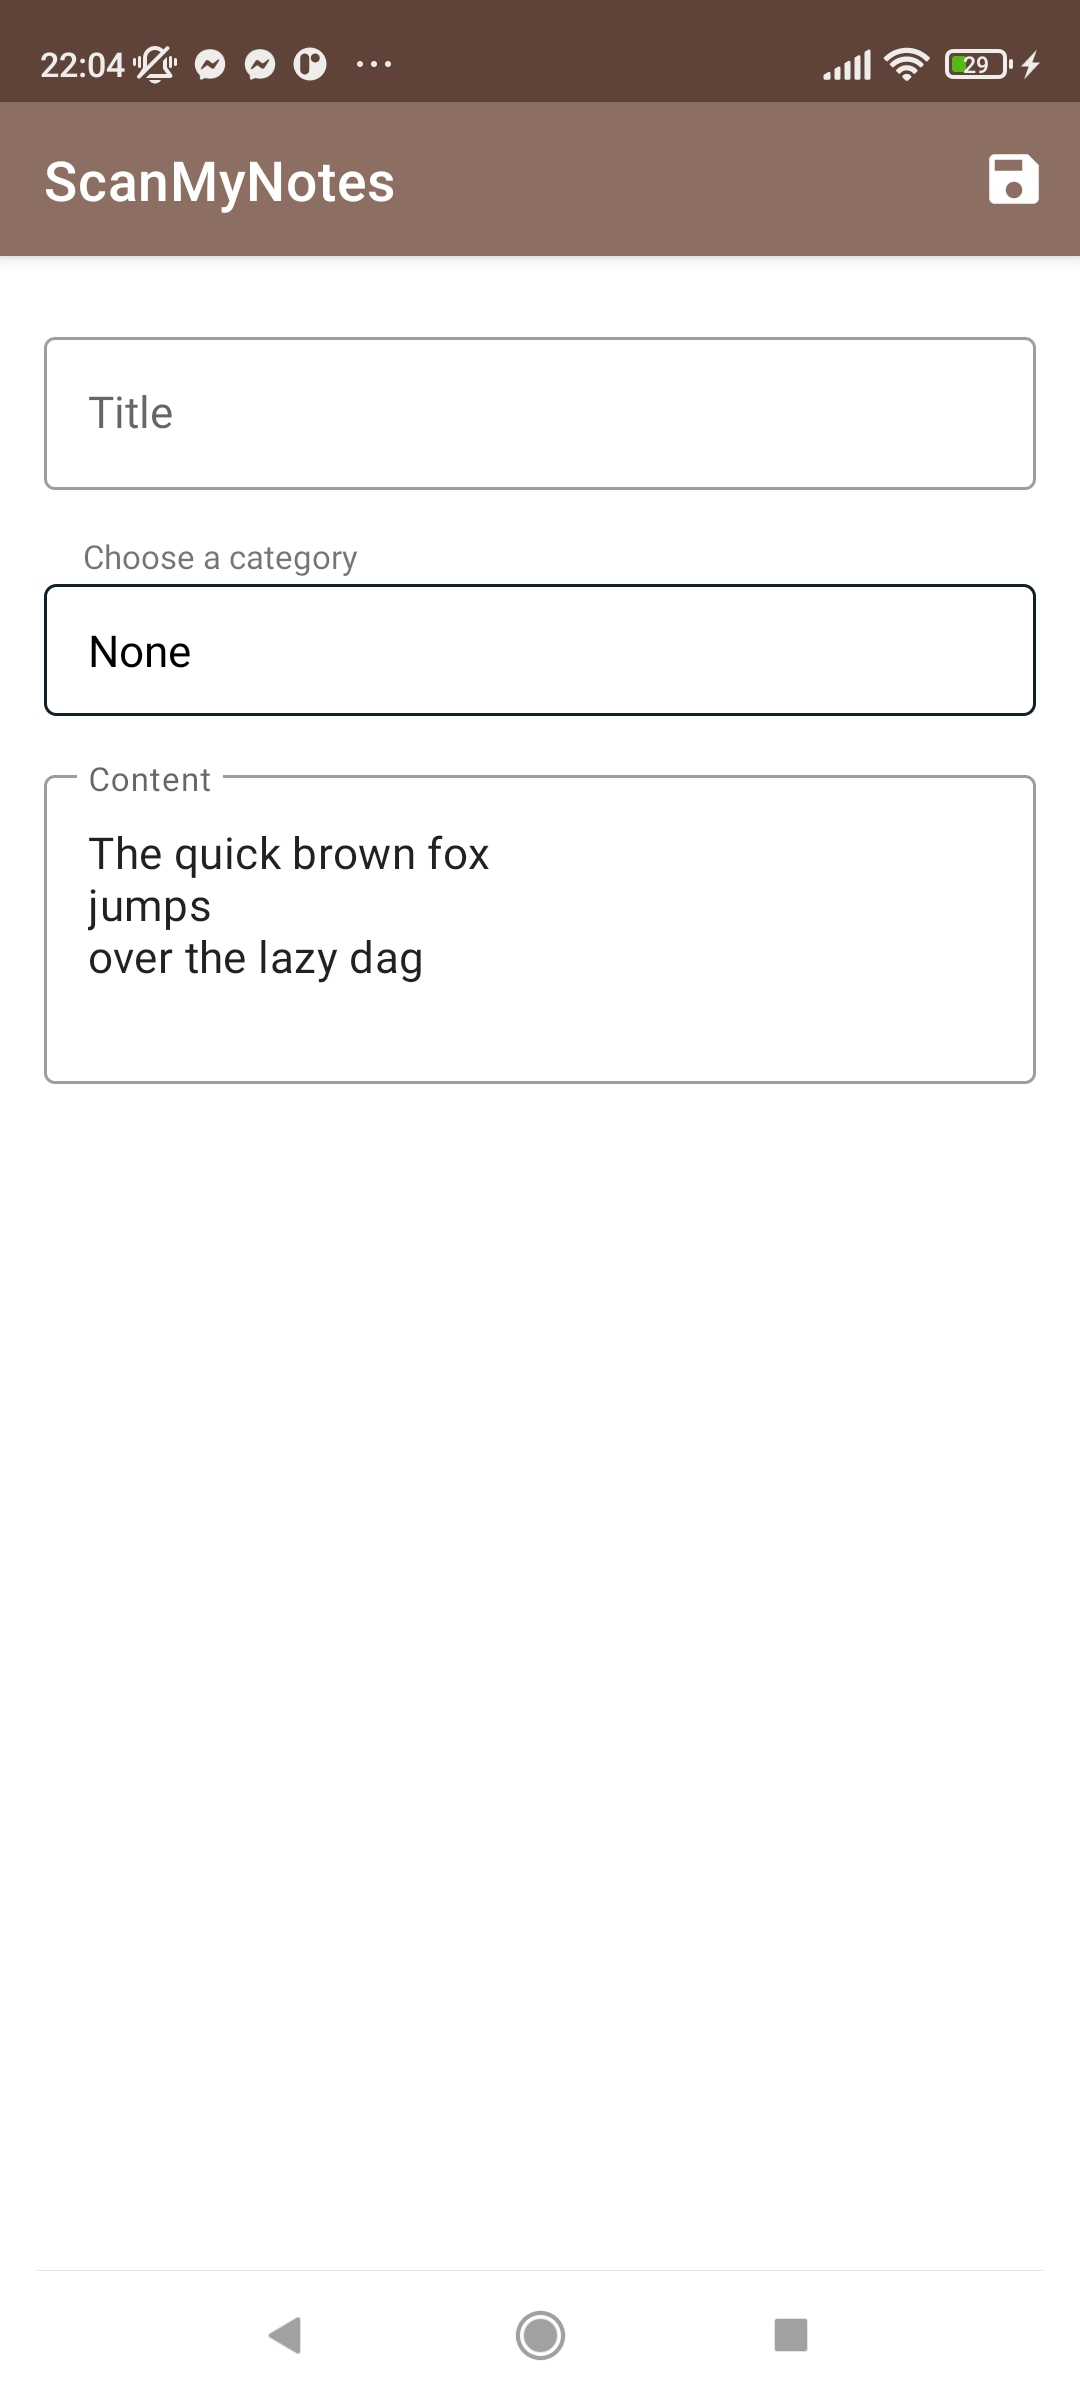
\includegraphics[width=55mm, keepaspectratio]{figures/newnote_create.jpg}
	\caption{A létrehozás során készített kép, illetve az abból kialakuló jegyzet szerkesztése.}
	\label{fig:NewNoteScreen}
\end{figure}

\section{Jegyzet szerkesztése}
Amennyiben a listában egy jegyzetre kattintunk, illetve újat hozunk létre, akkor annak részletes oldalára navigálunk. Itt megtekinthetjük a tartalmát, a jobb felső sarokban található ceruza ikonra nyomva pedig szerkeszthetjük is (\refstruc{fig:NoteDetailsScreen}). Megváltoztathatjuk a címét, tartalmát, kategóriáját, a fent megjelenő pluszjel segítségével pedig készíthetünk újabb fotót, melynek szövege hozzáfűzésre kerül az eddigihez. A fentebb említett megkötések itt is érvényesek, azaz a cím és a tartalom nem lehet üres az elmentés pillanatában.

Mind megtekintési, mind szerkesztési módban elérhető a fenti sávban a szemetes ikon, mellyel törölhetjük a jegyzetet a listánkból. Vigyázat, ez a művelet nem visszafordítható!

\begin{figure}[!ht]
	\centering
	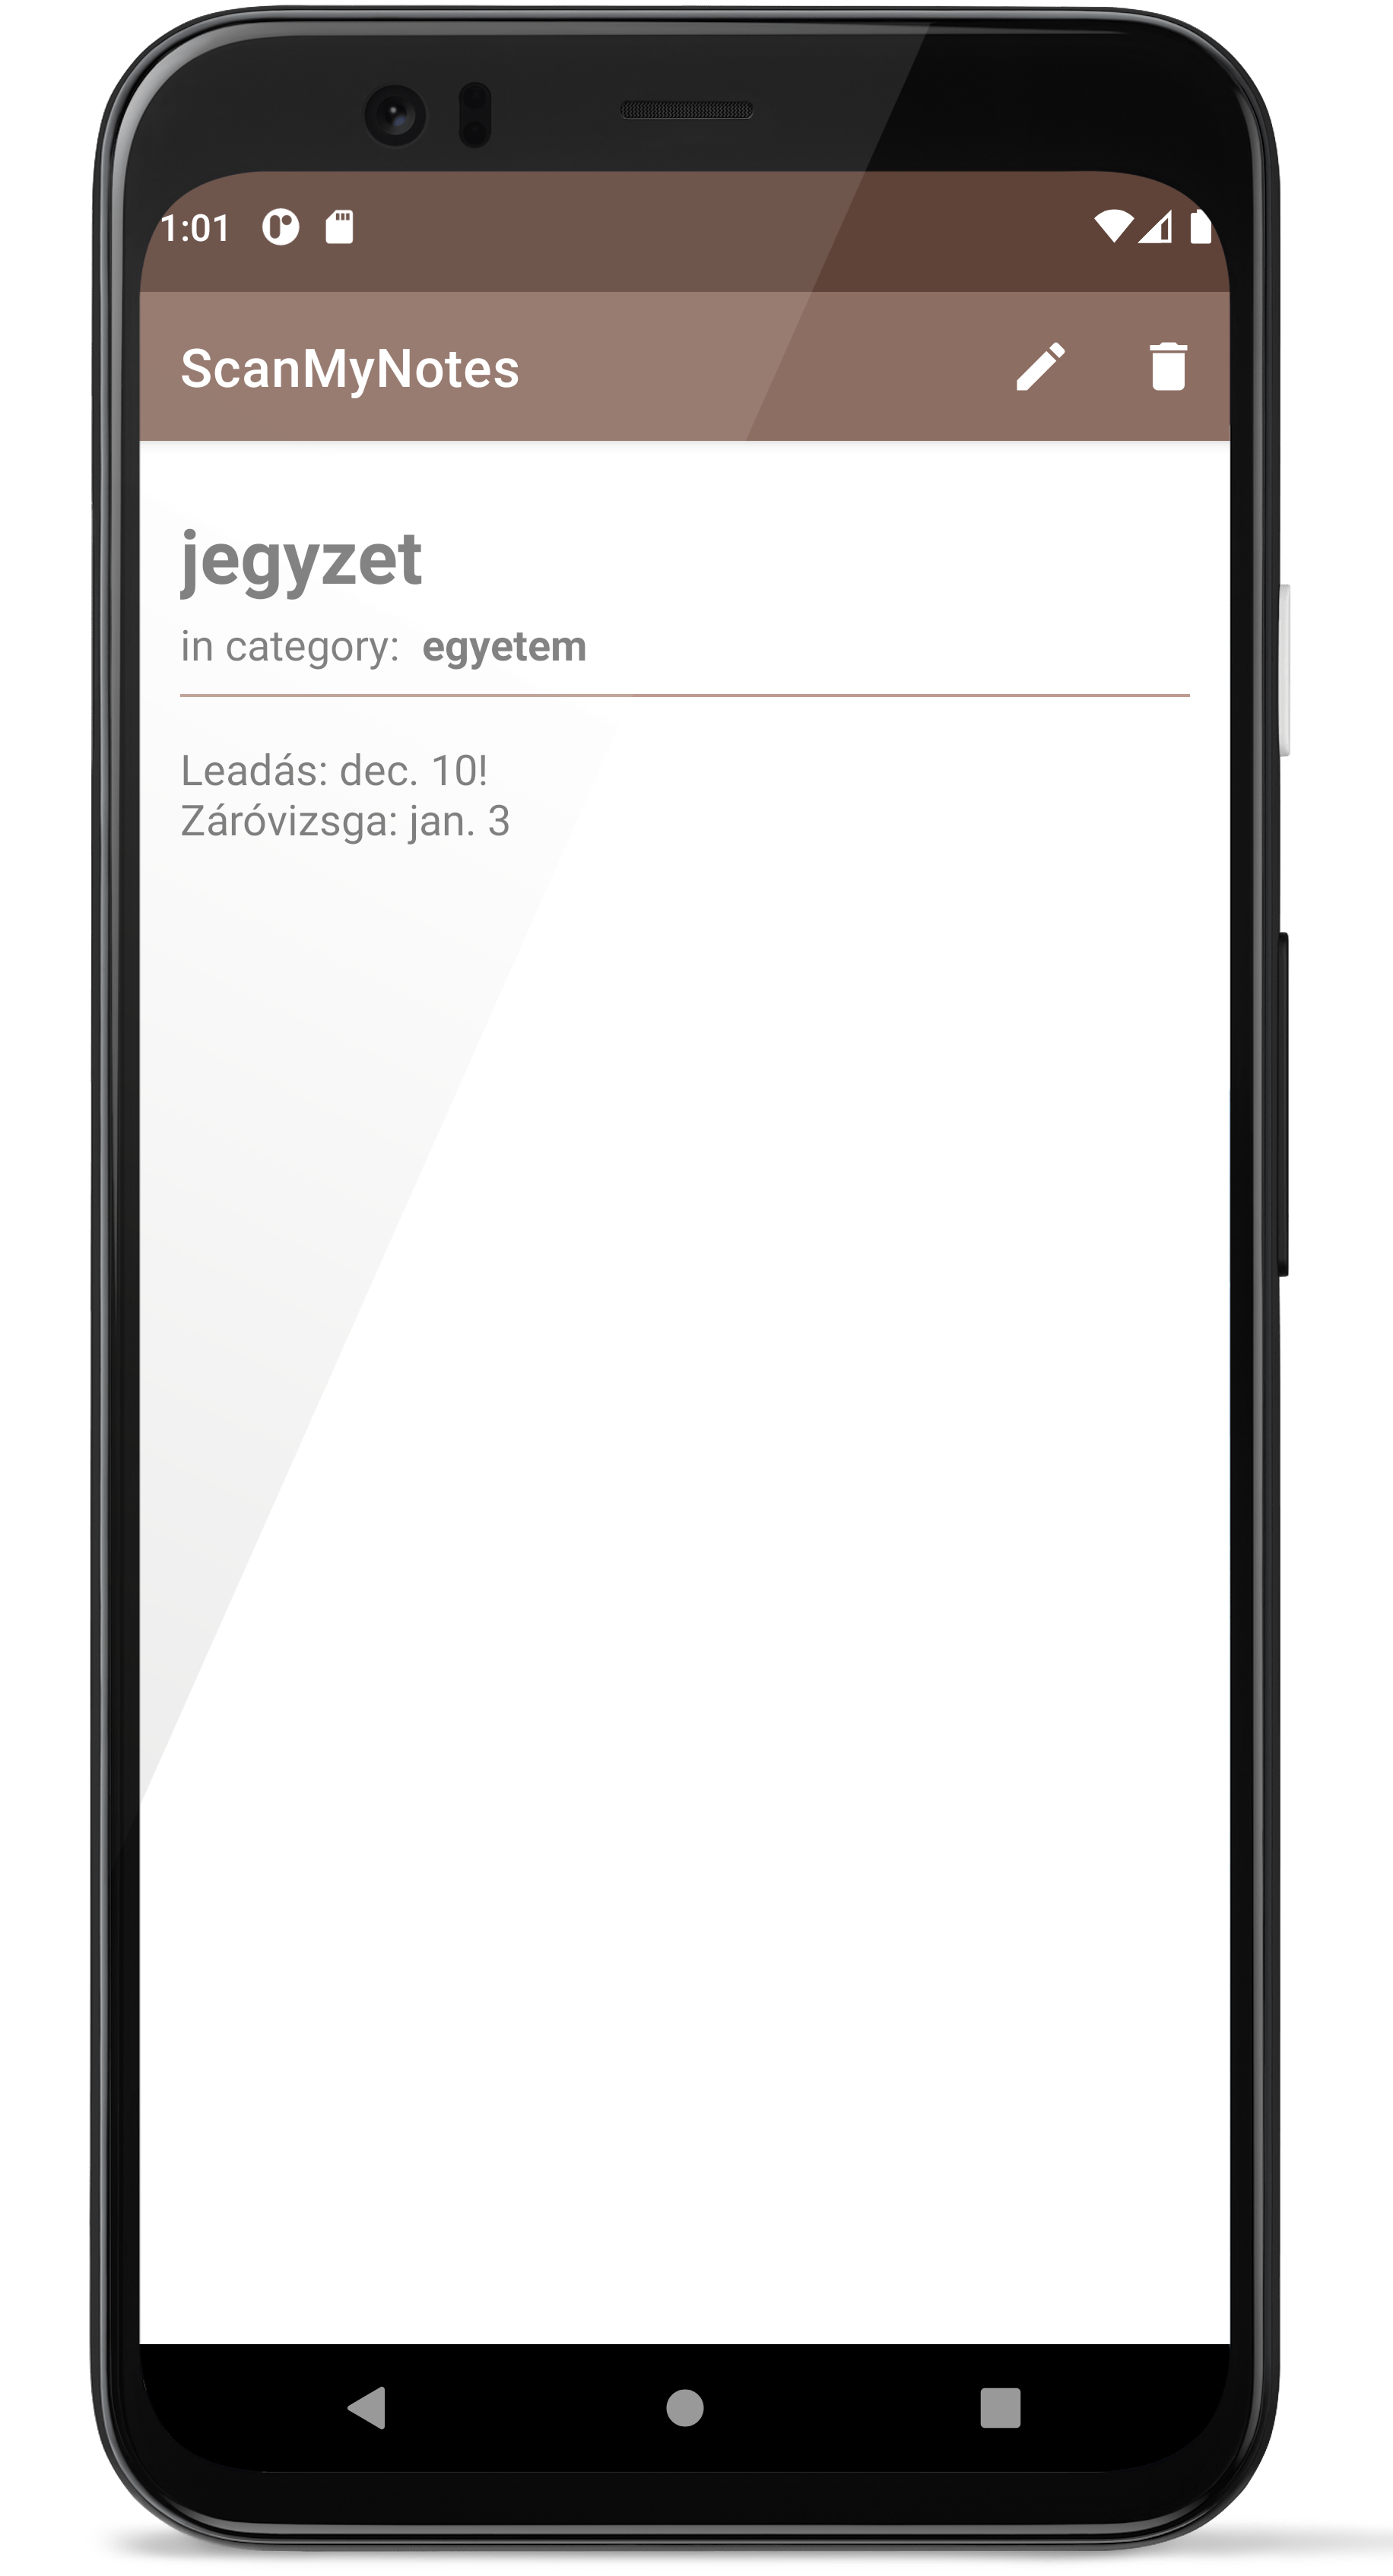
\includegraphics[width=55mm, keepaspectratio]{figures/note_view.png}
	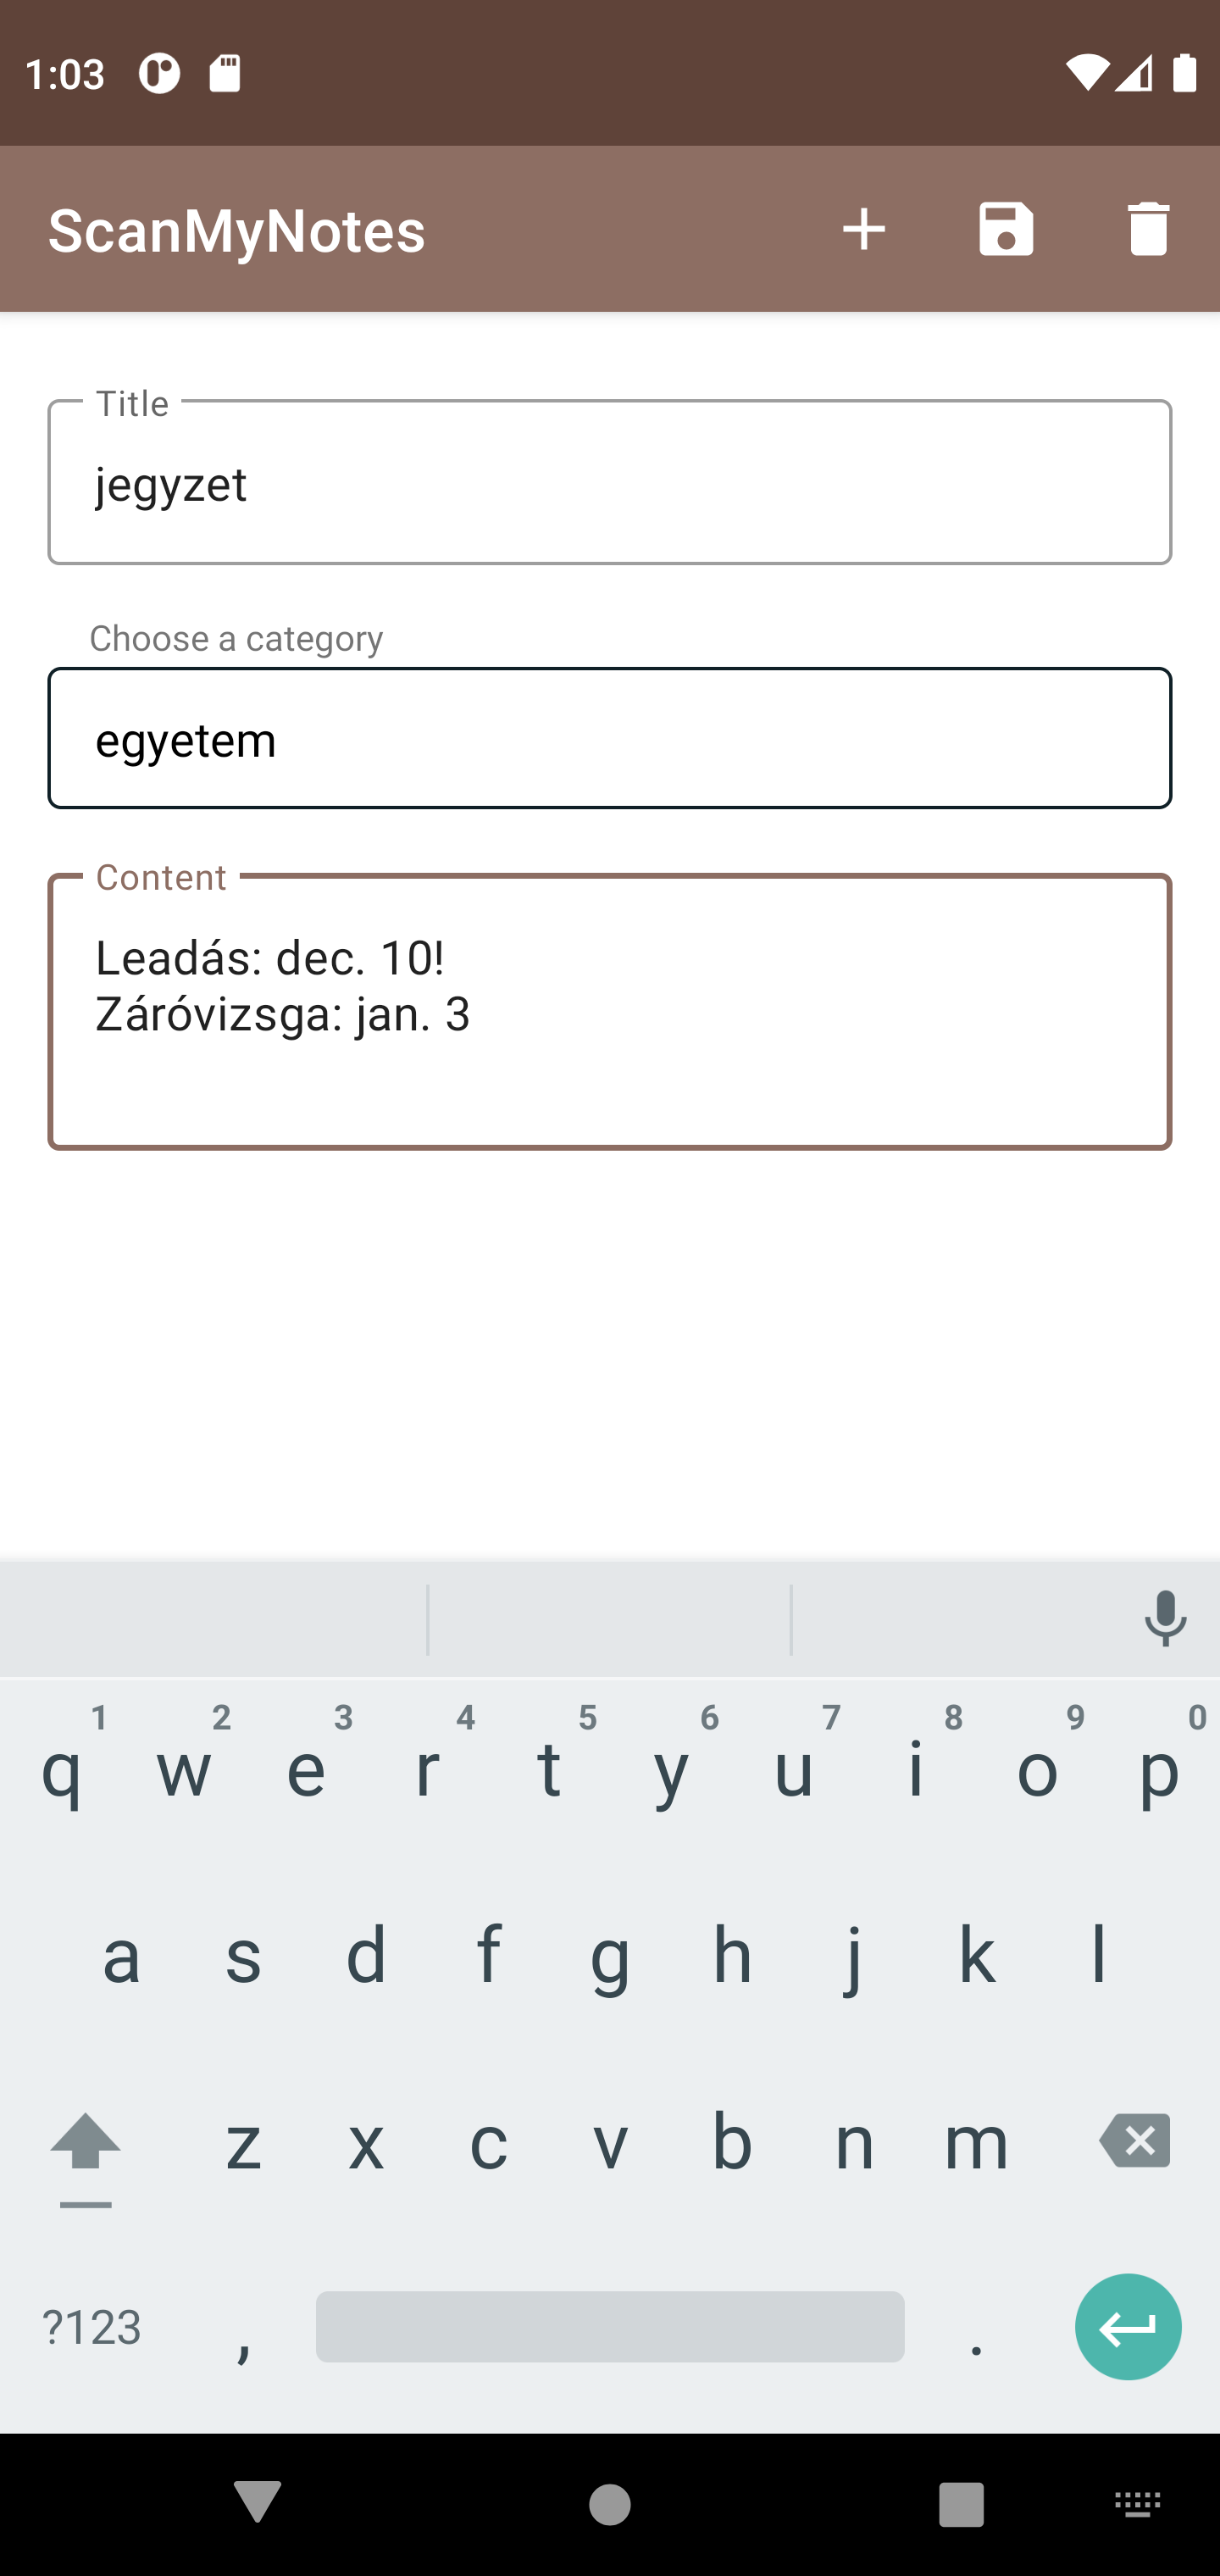
\includegraphics[width=55mm, keepaspectratio]{figures/note_edit.png}
	\caption{A jegyzet megtekintési, illetve szerkesztési képernyője.}
	\label{fig:NoteDetailsScreen}
\end{figure}

\section{Kategória létrehozása}
Az alkalmazásban elérhető másik adattípus a kategória, mely rendszerezési célt szolgál. Képes magába foglalni jegyzeteket és más kategóriákat is, tetszőleges mélységben. Szintén a jobb alsó sarokban található gomb biztosítja a létrehozás lehetőségét, ám ebben az esetben a felugró két kisebb gomb közül a felsőt kell választani. Itt egy, a jegyzetkészítéshez nagyon hasonló oldalon tudunk címet és opcionálisan szülőkategóriát megadni, és amennyiben nem üres a cím mezője, el is menthetjük (\refstruc{fig:NewCategoryScreen}).

\begin{figure}[!ht]
	\centering
	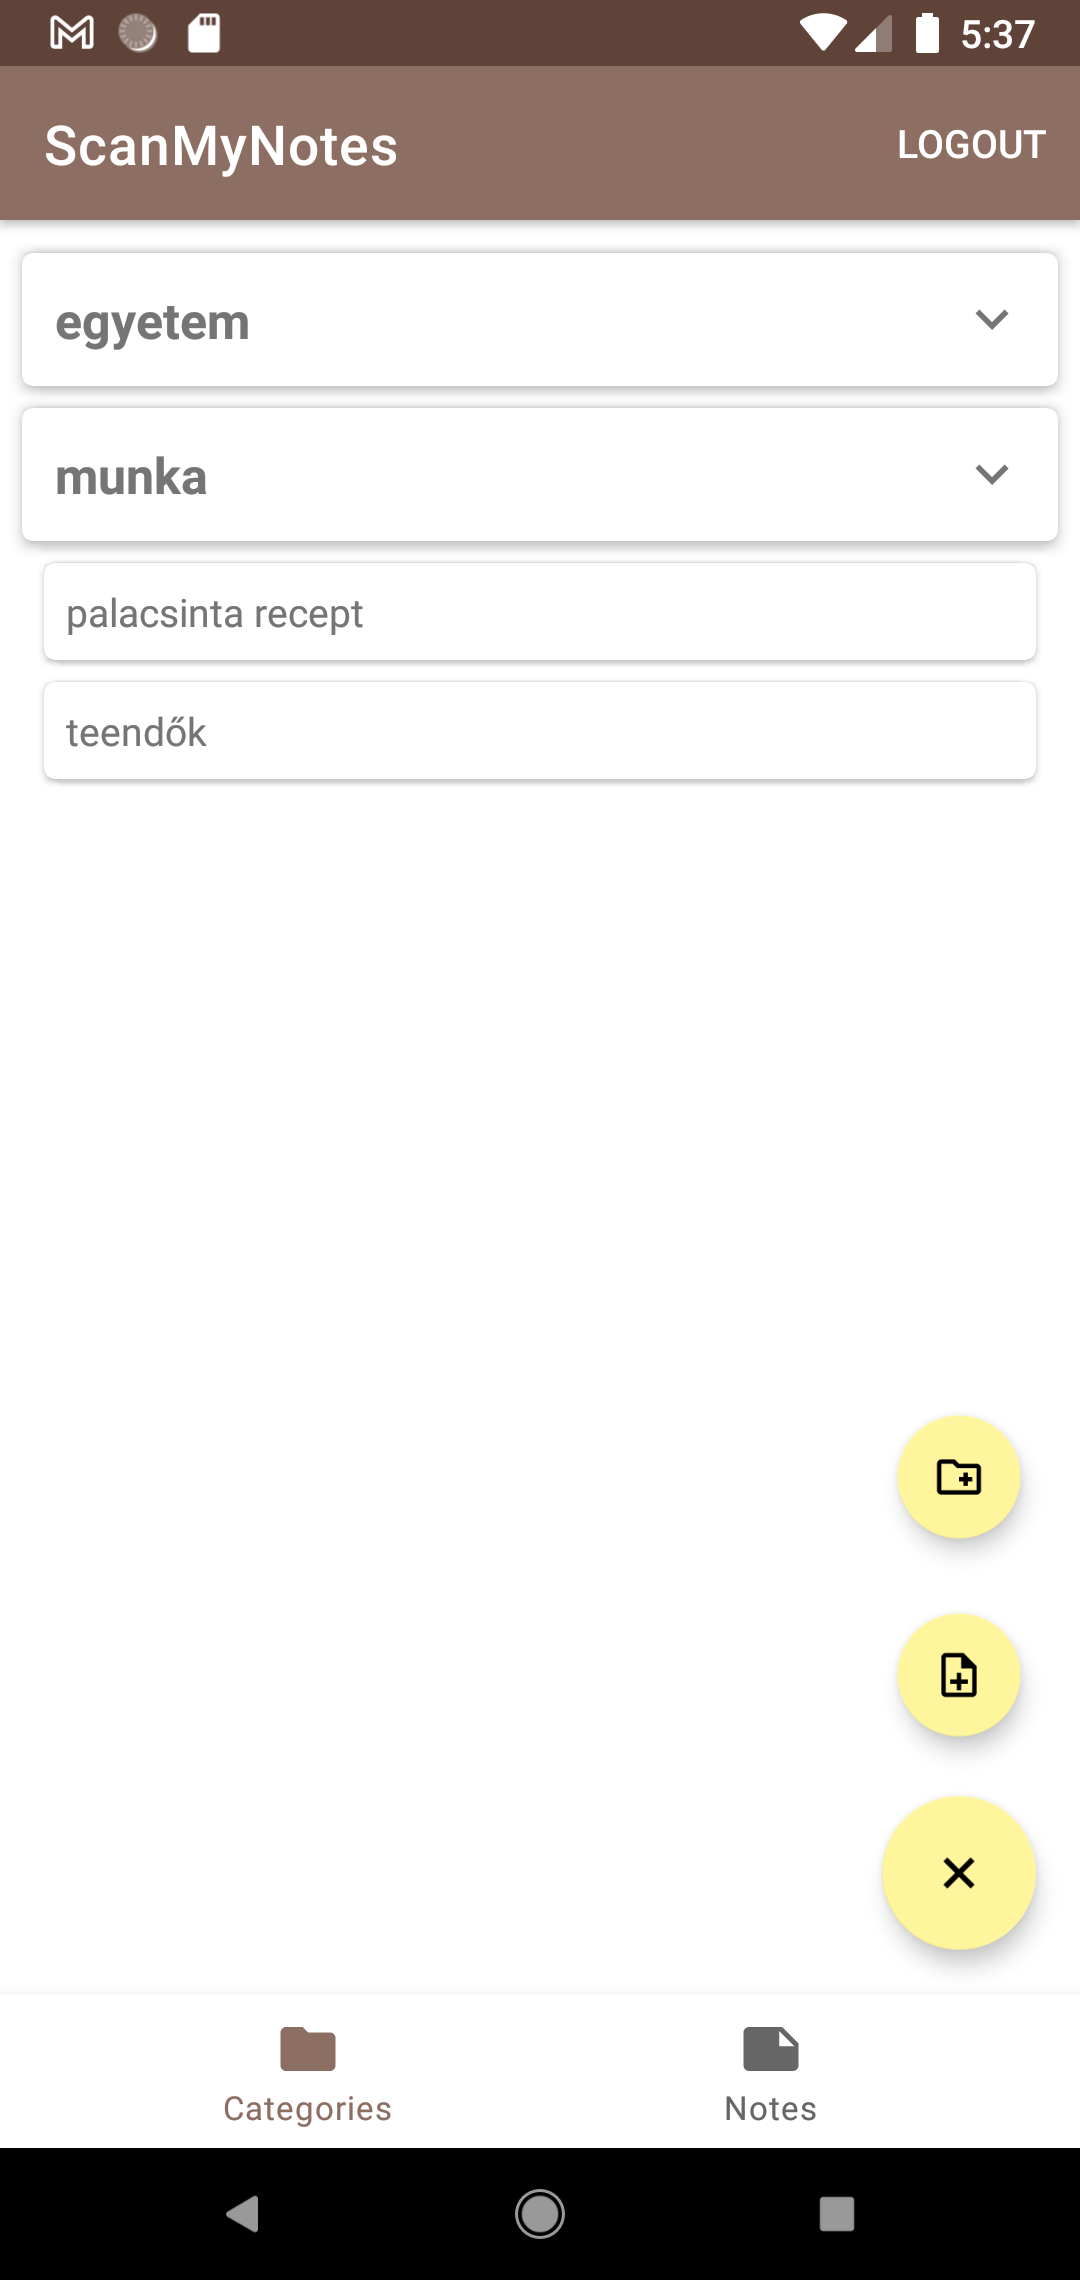
\includegraphics[width=50mm, keepaspectratio]{figures/floatingbutton_open.png}
	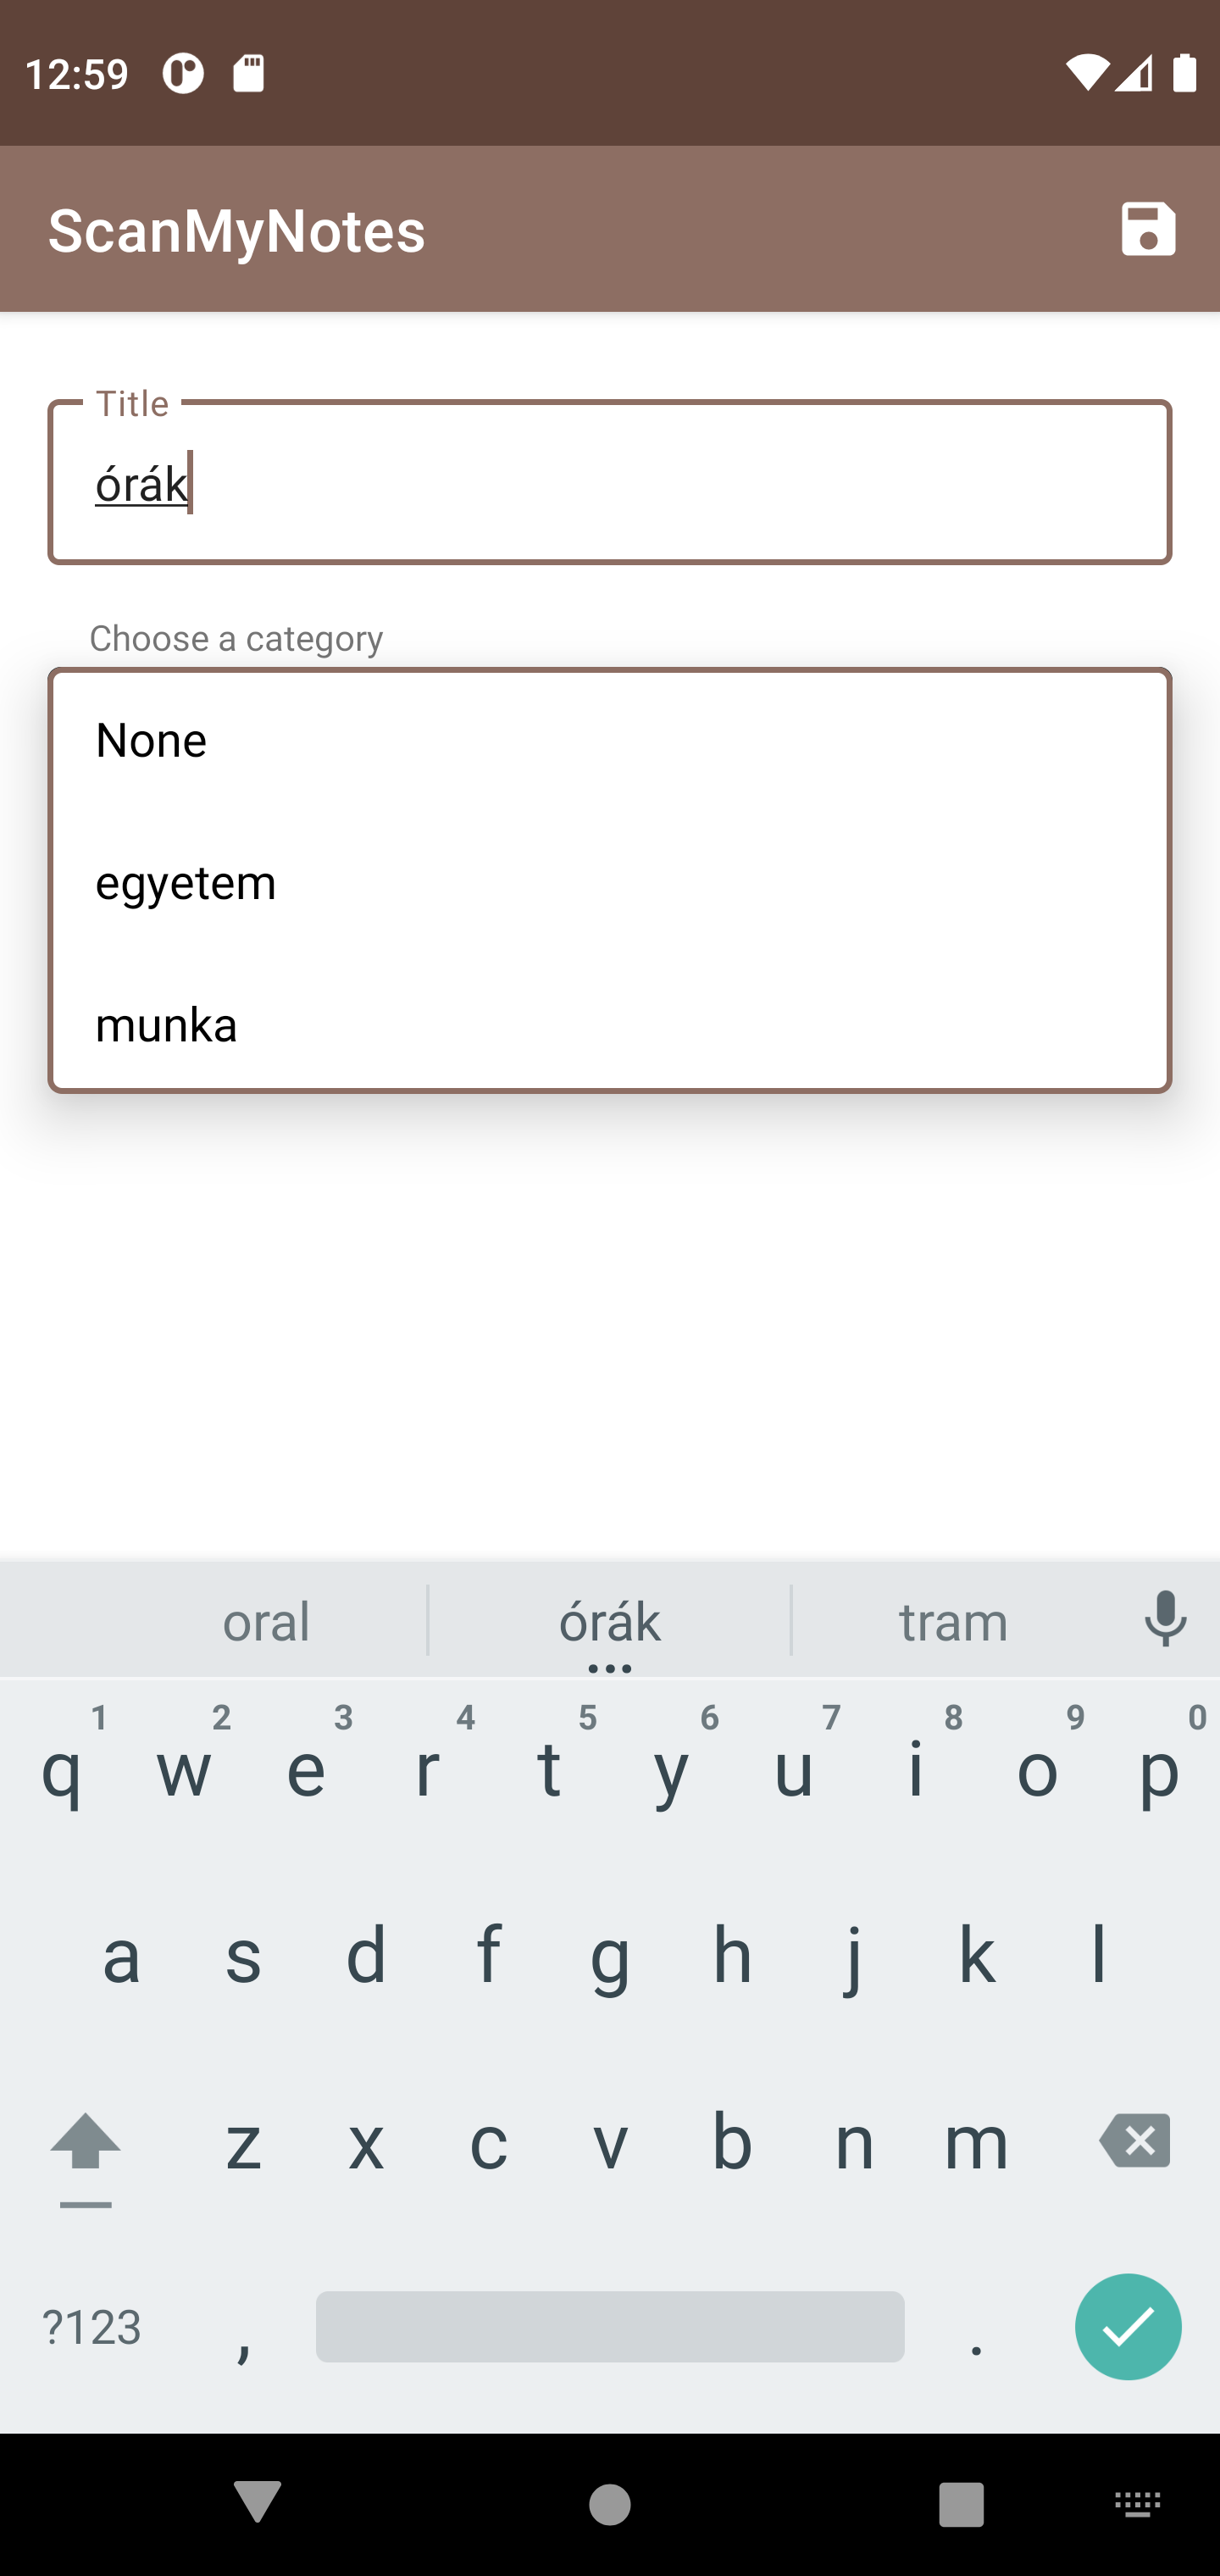
\includegraphics[width=50mm, keepaspectratio]{figures/category_save.png}
	\caption{A létrehozás gomb kinyitott állapotban, új kategória felvétele.}
	\label{fig:NewCategoryScreen}
\end{figure}

\section{Kategória szerkesztése}
Új kategória létrehozása után, illetve a listában egy kategóriára nyomva annak részleteit tekinthetjük meg. Itt megjelenik a címe és esetleges szülője, és jobb fent szintén található egy ceruza ikon, mely lehetővé teszi a szerkesztést (\refstruc{fig:CategoryDetailsScreen}). Hasonlóan a jegyzethez megtekintés és szerkesztés során is törölhetjük az adott kategóriát, ilyenkor egy felugró ablak figyelmeztet rá, hogy a törlés során az összes tartalmazott objektum is törlődni fog.

\begin{figure}[!ht]
	\centering
	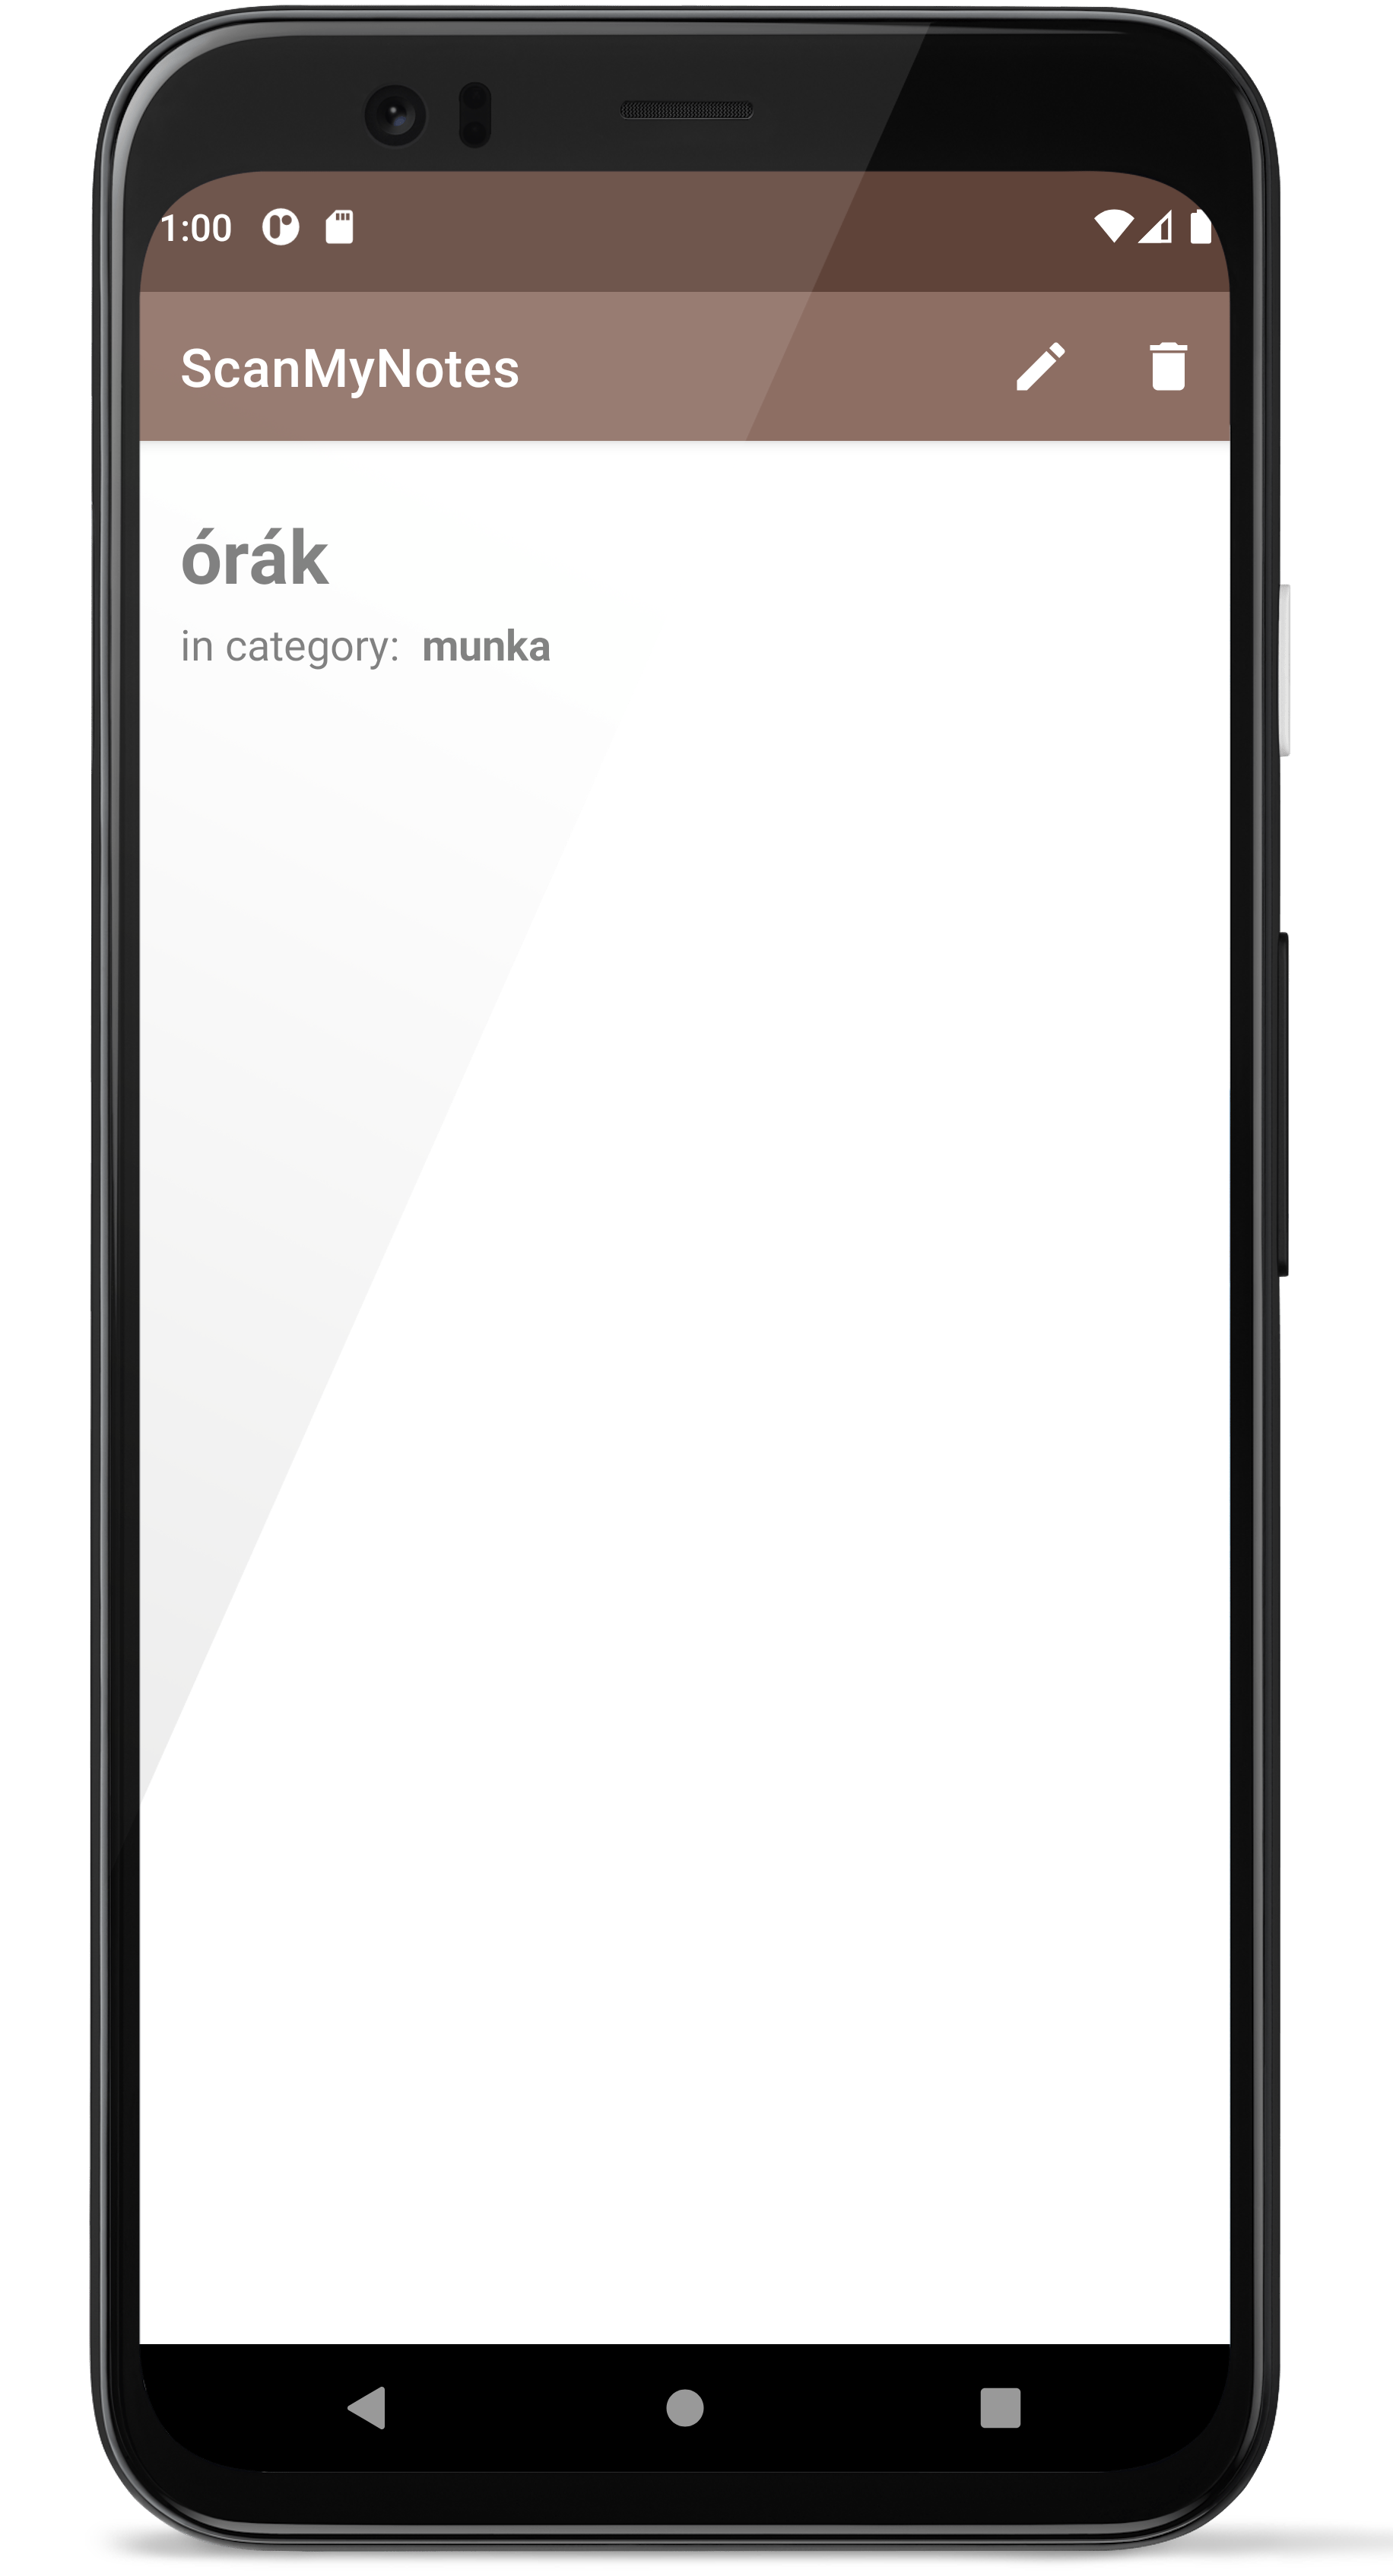
\includegraphics[width=50mm, keepaspectratio]{figures/category_view.png}
	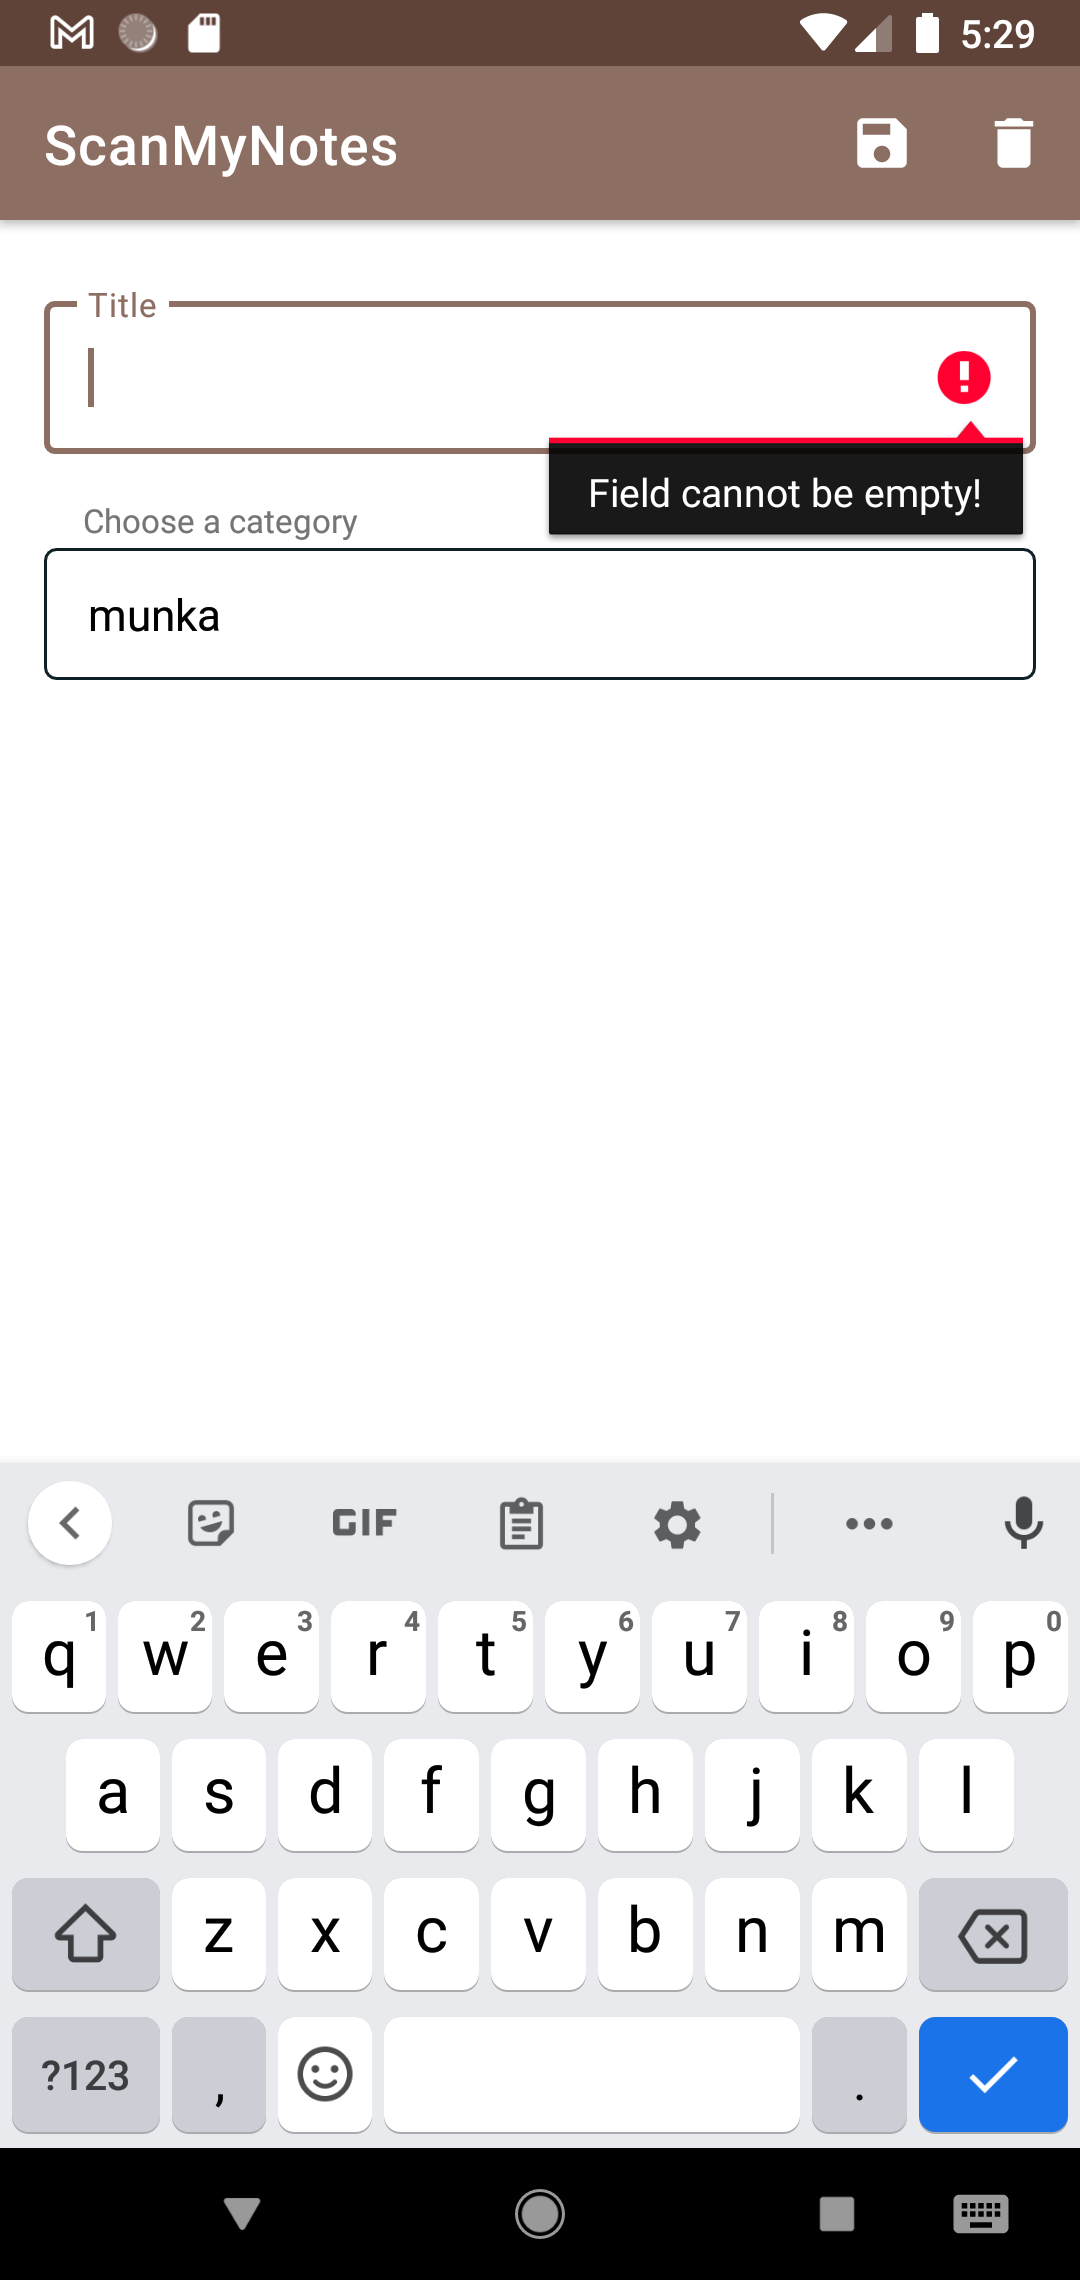
\includegraphics[width=50mm, keepaspectratio]{figures/category_edit_error.png}
	\caption{A kategória részletes képernyője, illetve a szerkesztési képernyő által feldobott hiba, ha üresen hagyjuk a címet.}
	\label{fig:CategoryDetailsScreen}
\end{figure}